\section{Results} \label{results}
In this Chapter, we will first describe the different models that are used for comparison, but not all models are used for every metric. The first metric we look at is geometry size as this was not the highest priority. Then we have a look at the effectiveness of block and clustering compression methods. These results all relate to requirements \nameref{requirements:asset_size} and \nameref{requirements:lossy_compression}. Lastly we cover the ray tracing performance which deals with \nameref{requirements:sampling_speed}. The two requirements that will not have results attached to them are \nameref{requirements:level_of_detail} and \nameref{requirements:animation_playback}. The former was not implemented but can be added, and the latter is practically free as we use flip book animations where we only have to update a single index to switch between animation frames.


\subsection{Models} \label{results:models}
Multiple models were used to evaluate the implemented methods in Chapter \ref{implementation}. The model with the largest scale is the Disney Cloud \cite{DisneyCloud}. Our implementation is bound by volumes with size $4096^3$, so we use the half-resolution version. We also use multiple models from the \href{https://www.openvdb.org/download/}{OpenVDB website} and the \href{https://jangafx.com/software/embergen/download/free-vdb-animations/}{JangaFX website}. A mix of models was used with diverse axis sizes, number of voxels, animation frame numbers and shapes. Most models are static and thus consist of only a single animation frame, but to get a rough idea of the scaling of our structure size with the number of animation frames, we specifically used models with 10, 50 and 100 frames as well.

\begin{figure}[H]
    \centering
    \subfloat[Fire]{
        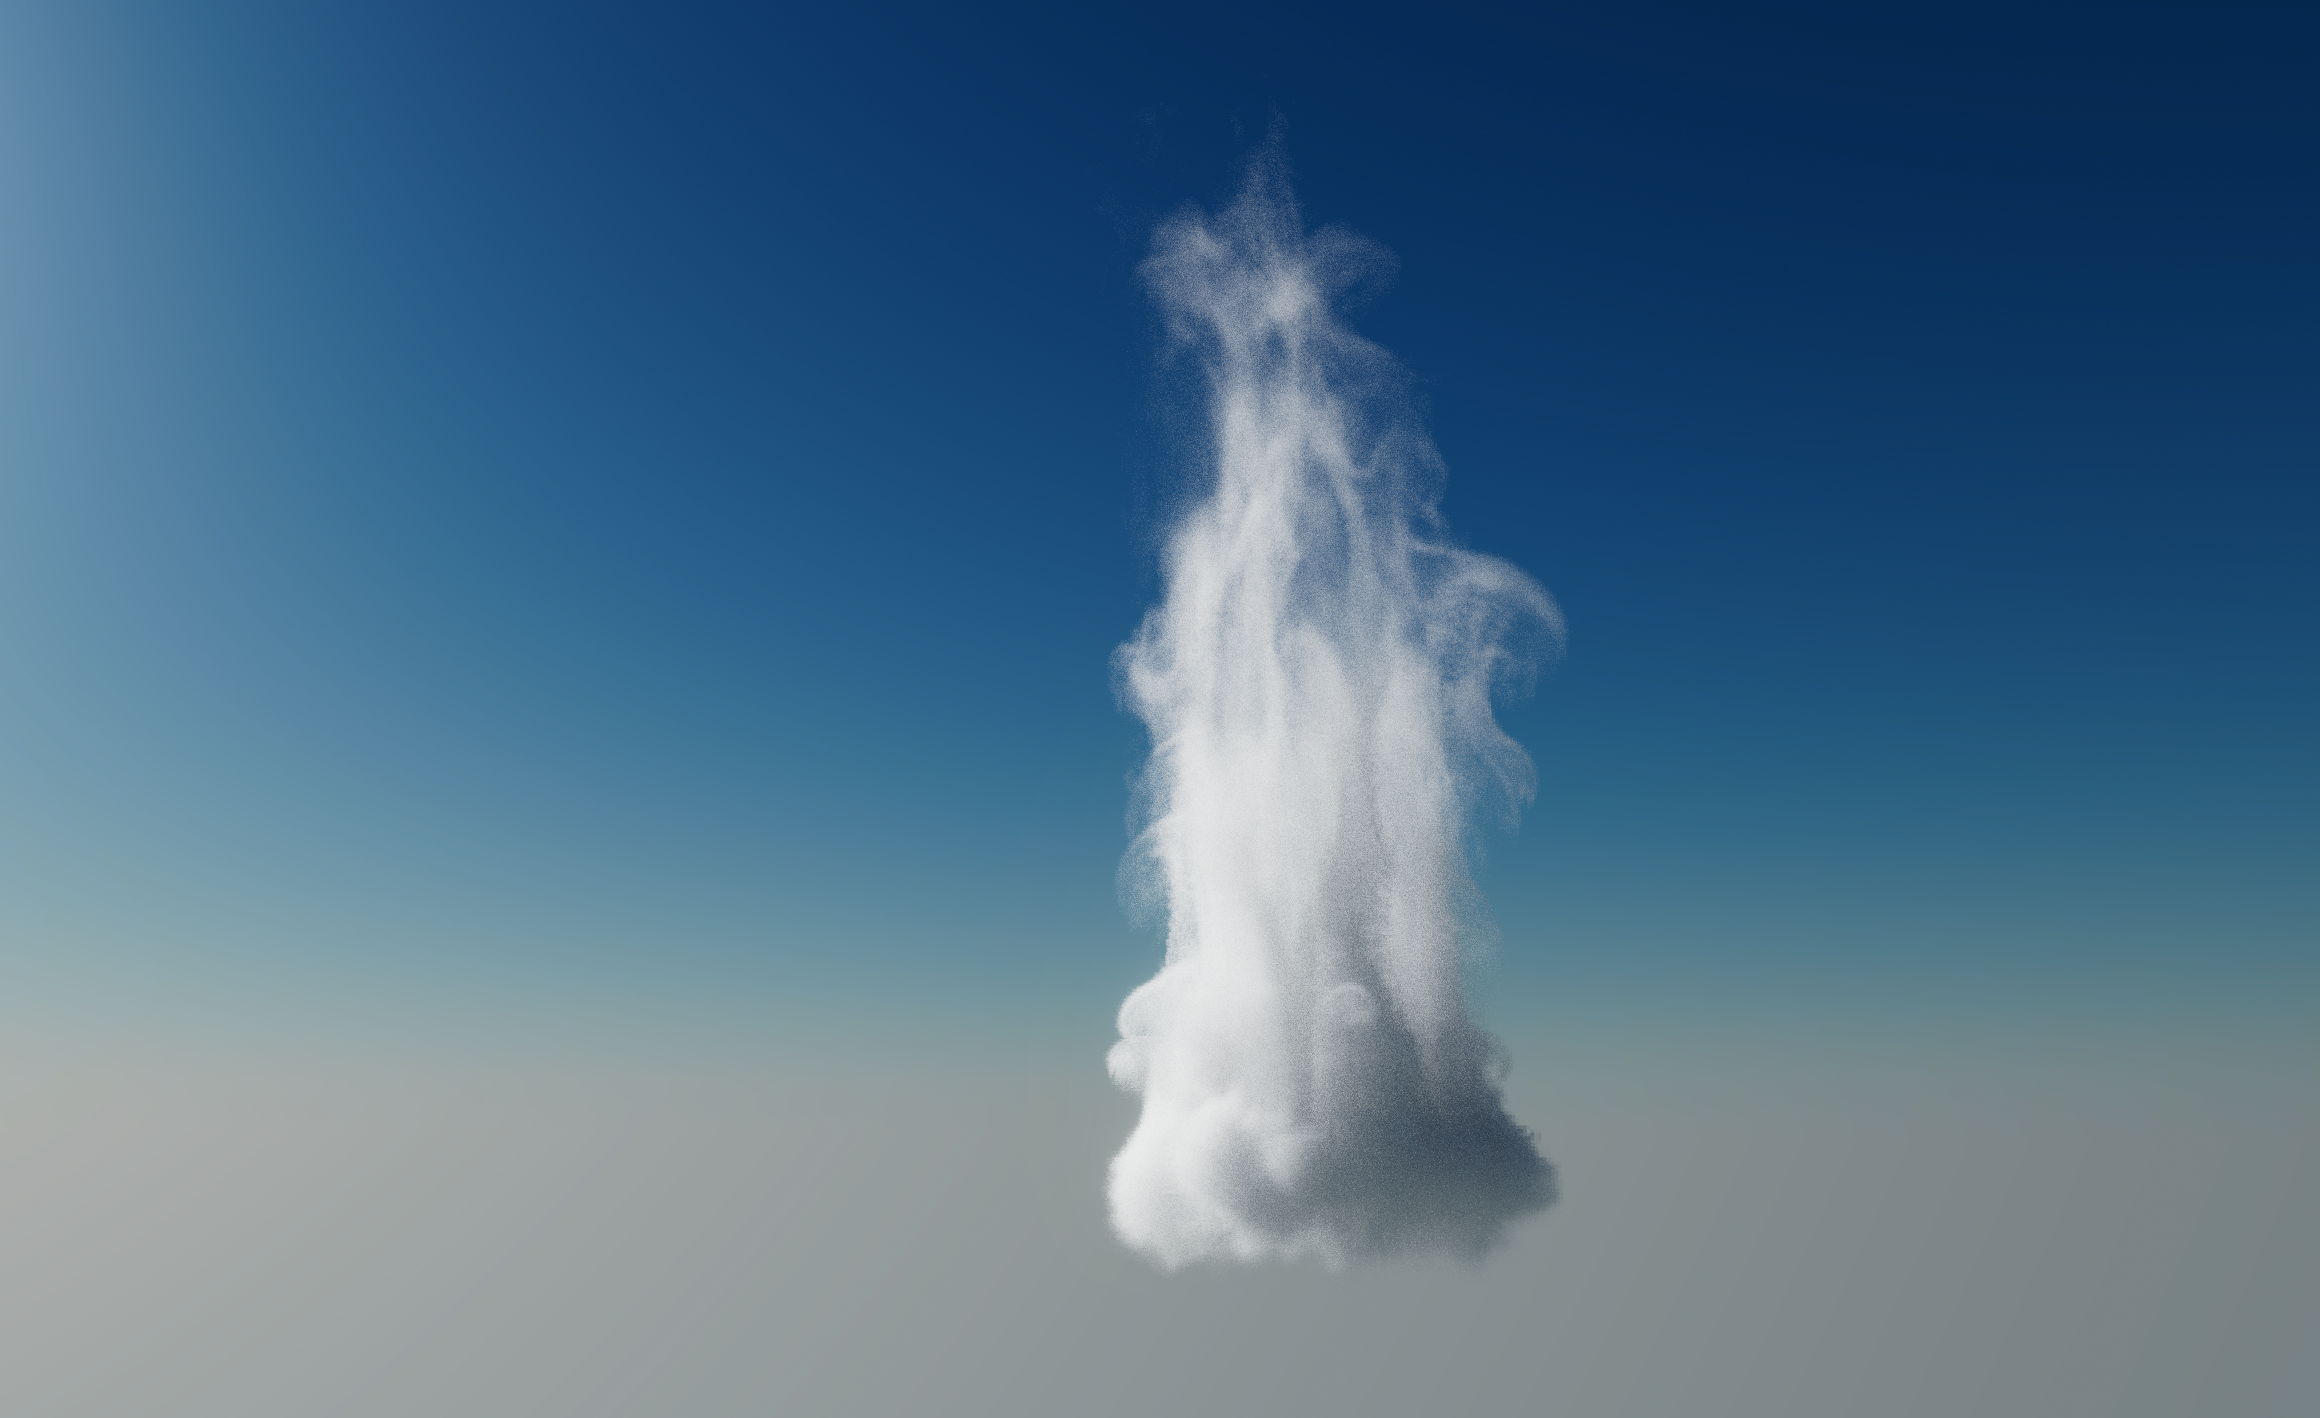
\includegraphics[width=0.3\textwidth]{figures/fire.png}
    }
    \hfill
    \subfloat[Bunny]{
        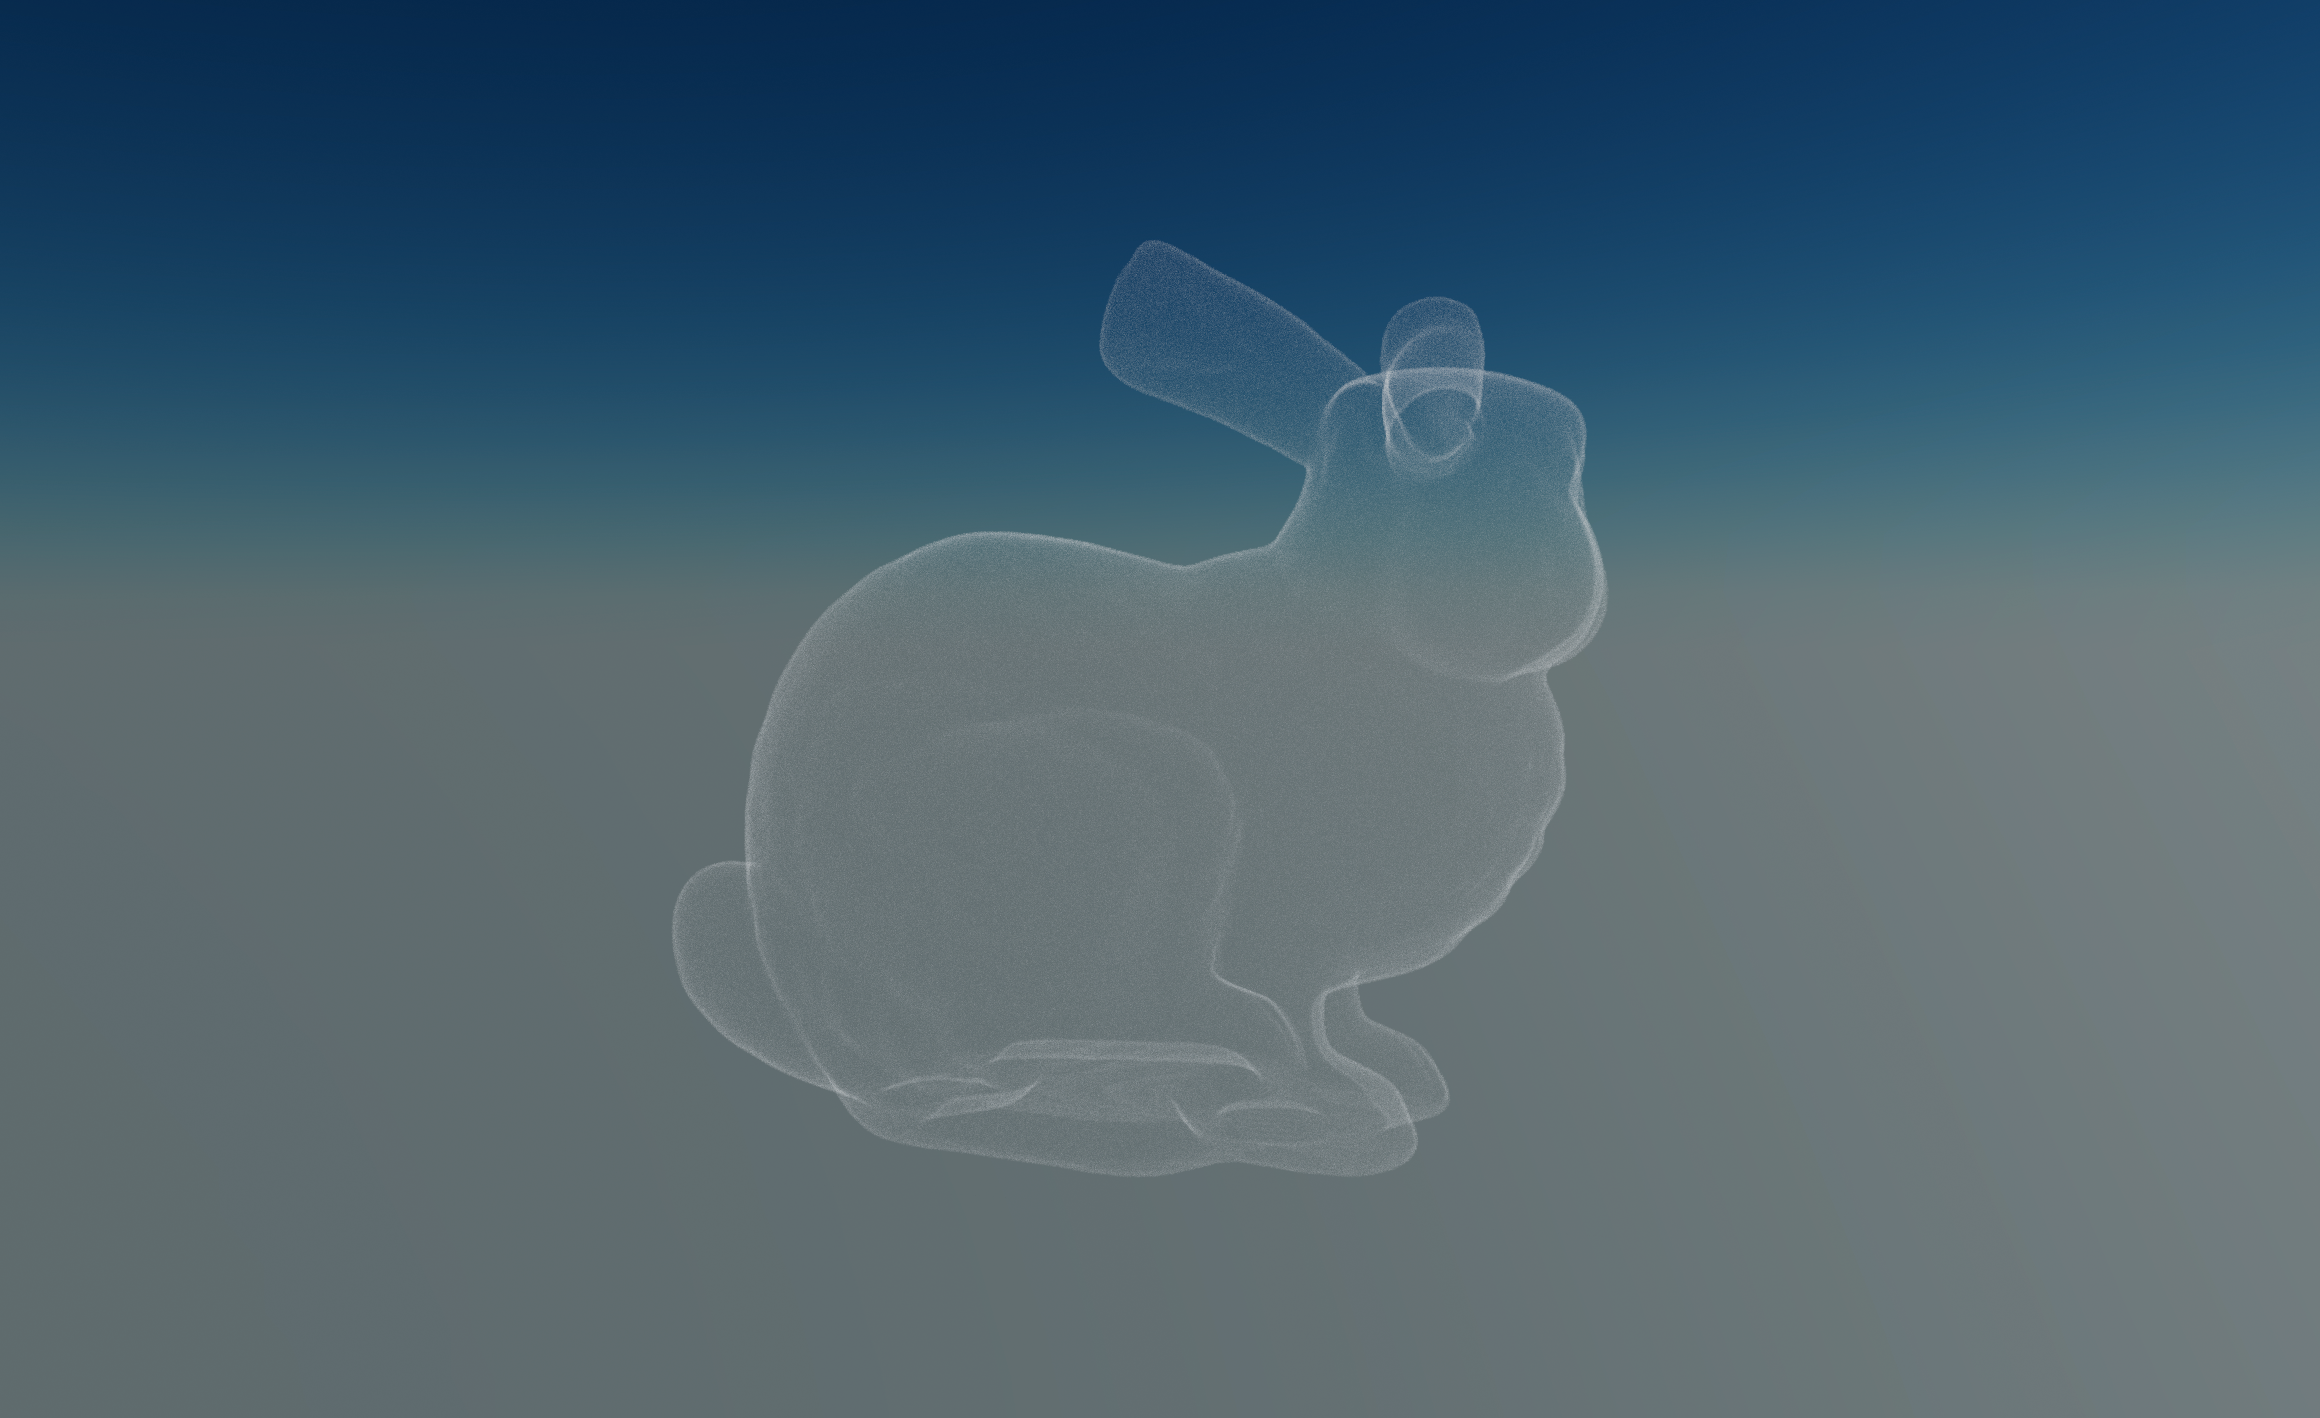
\includegraphics[width=0.3\textwidth]{figures/bunny.png}
    }
    \hfill
    \subfloat[Bunny cloud]{
        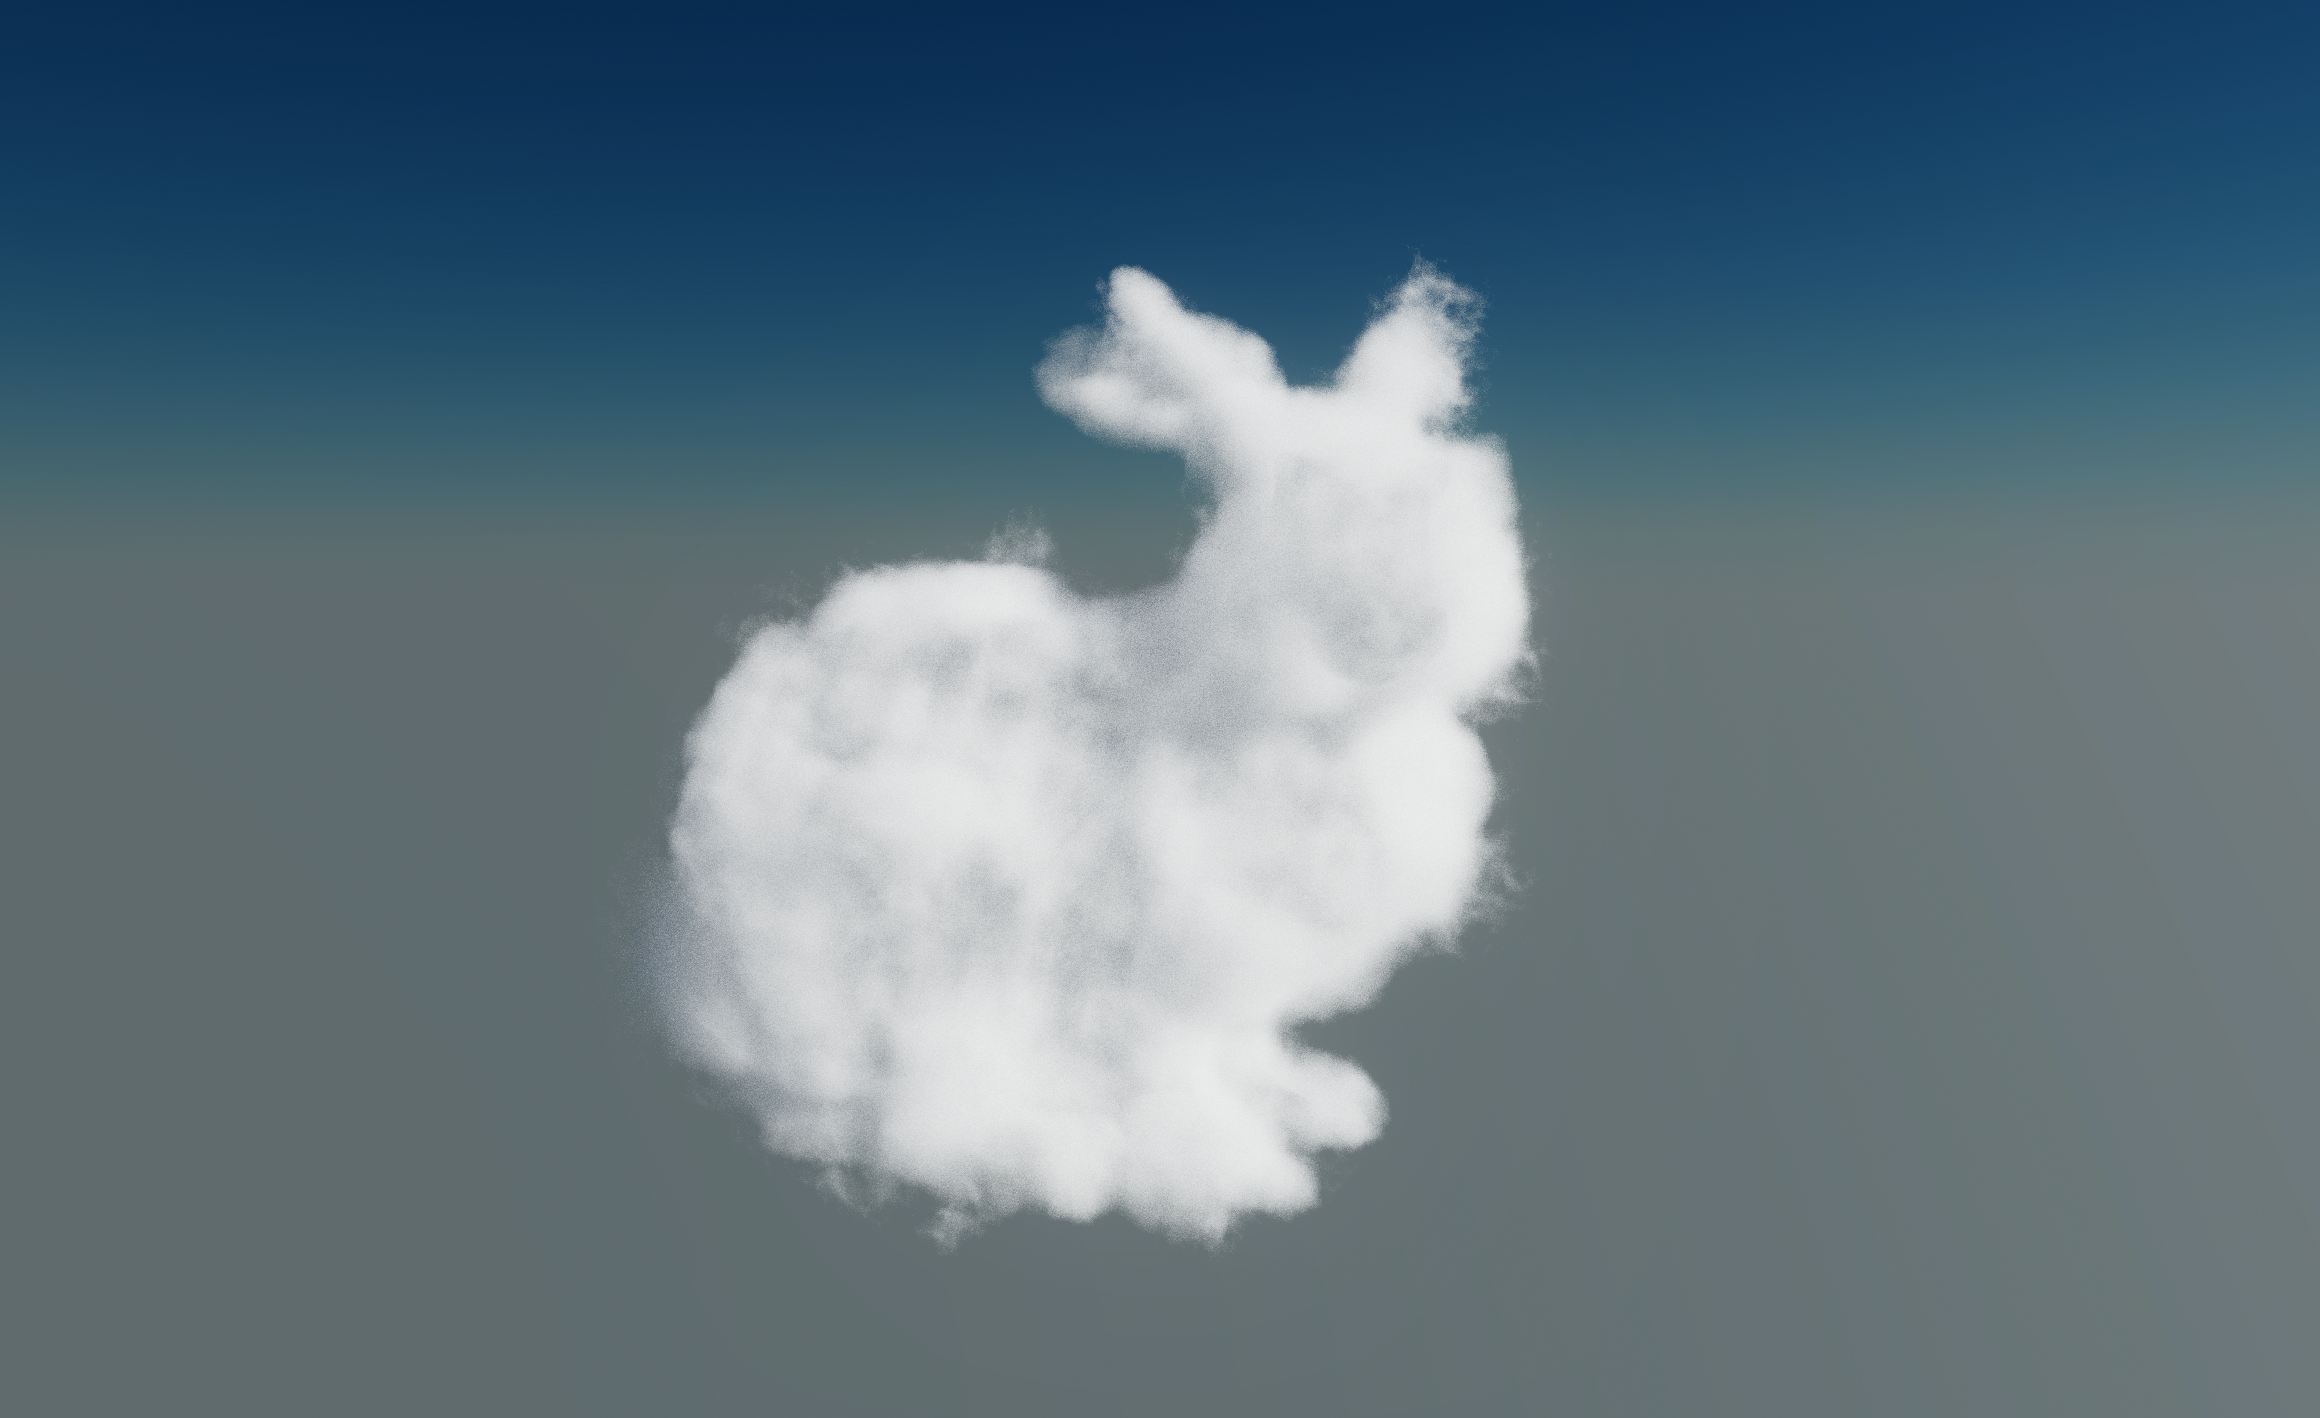
\includegraphics[width=0.3\textwidth]{figures/bunny cloud.png}
    }
    \hfill
    \subfloat[Armadillo]{
        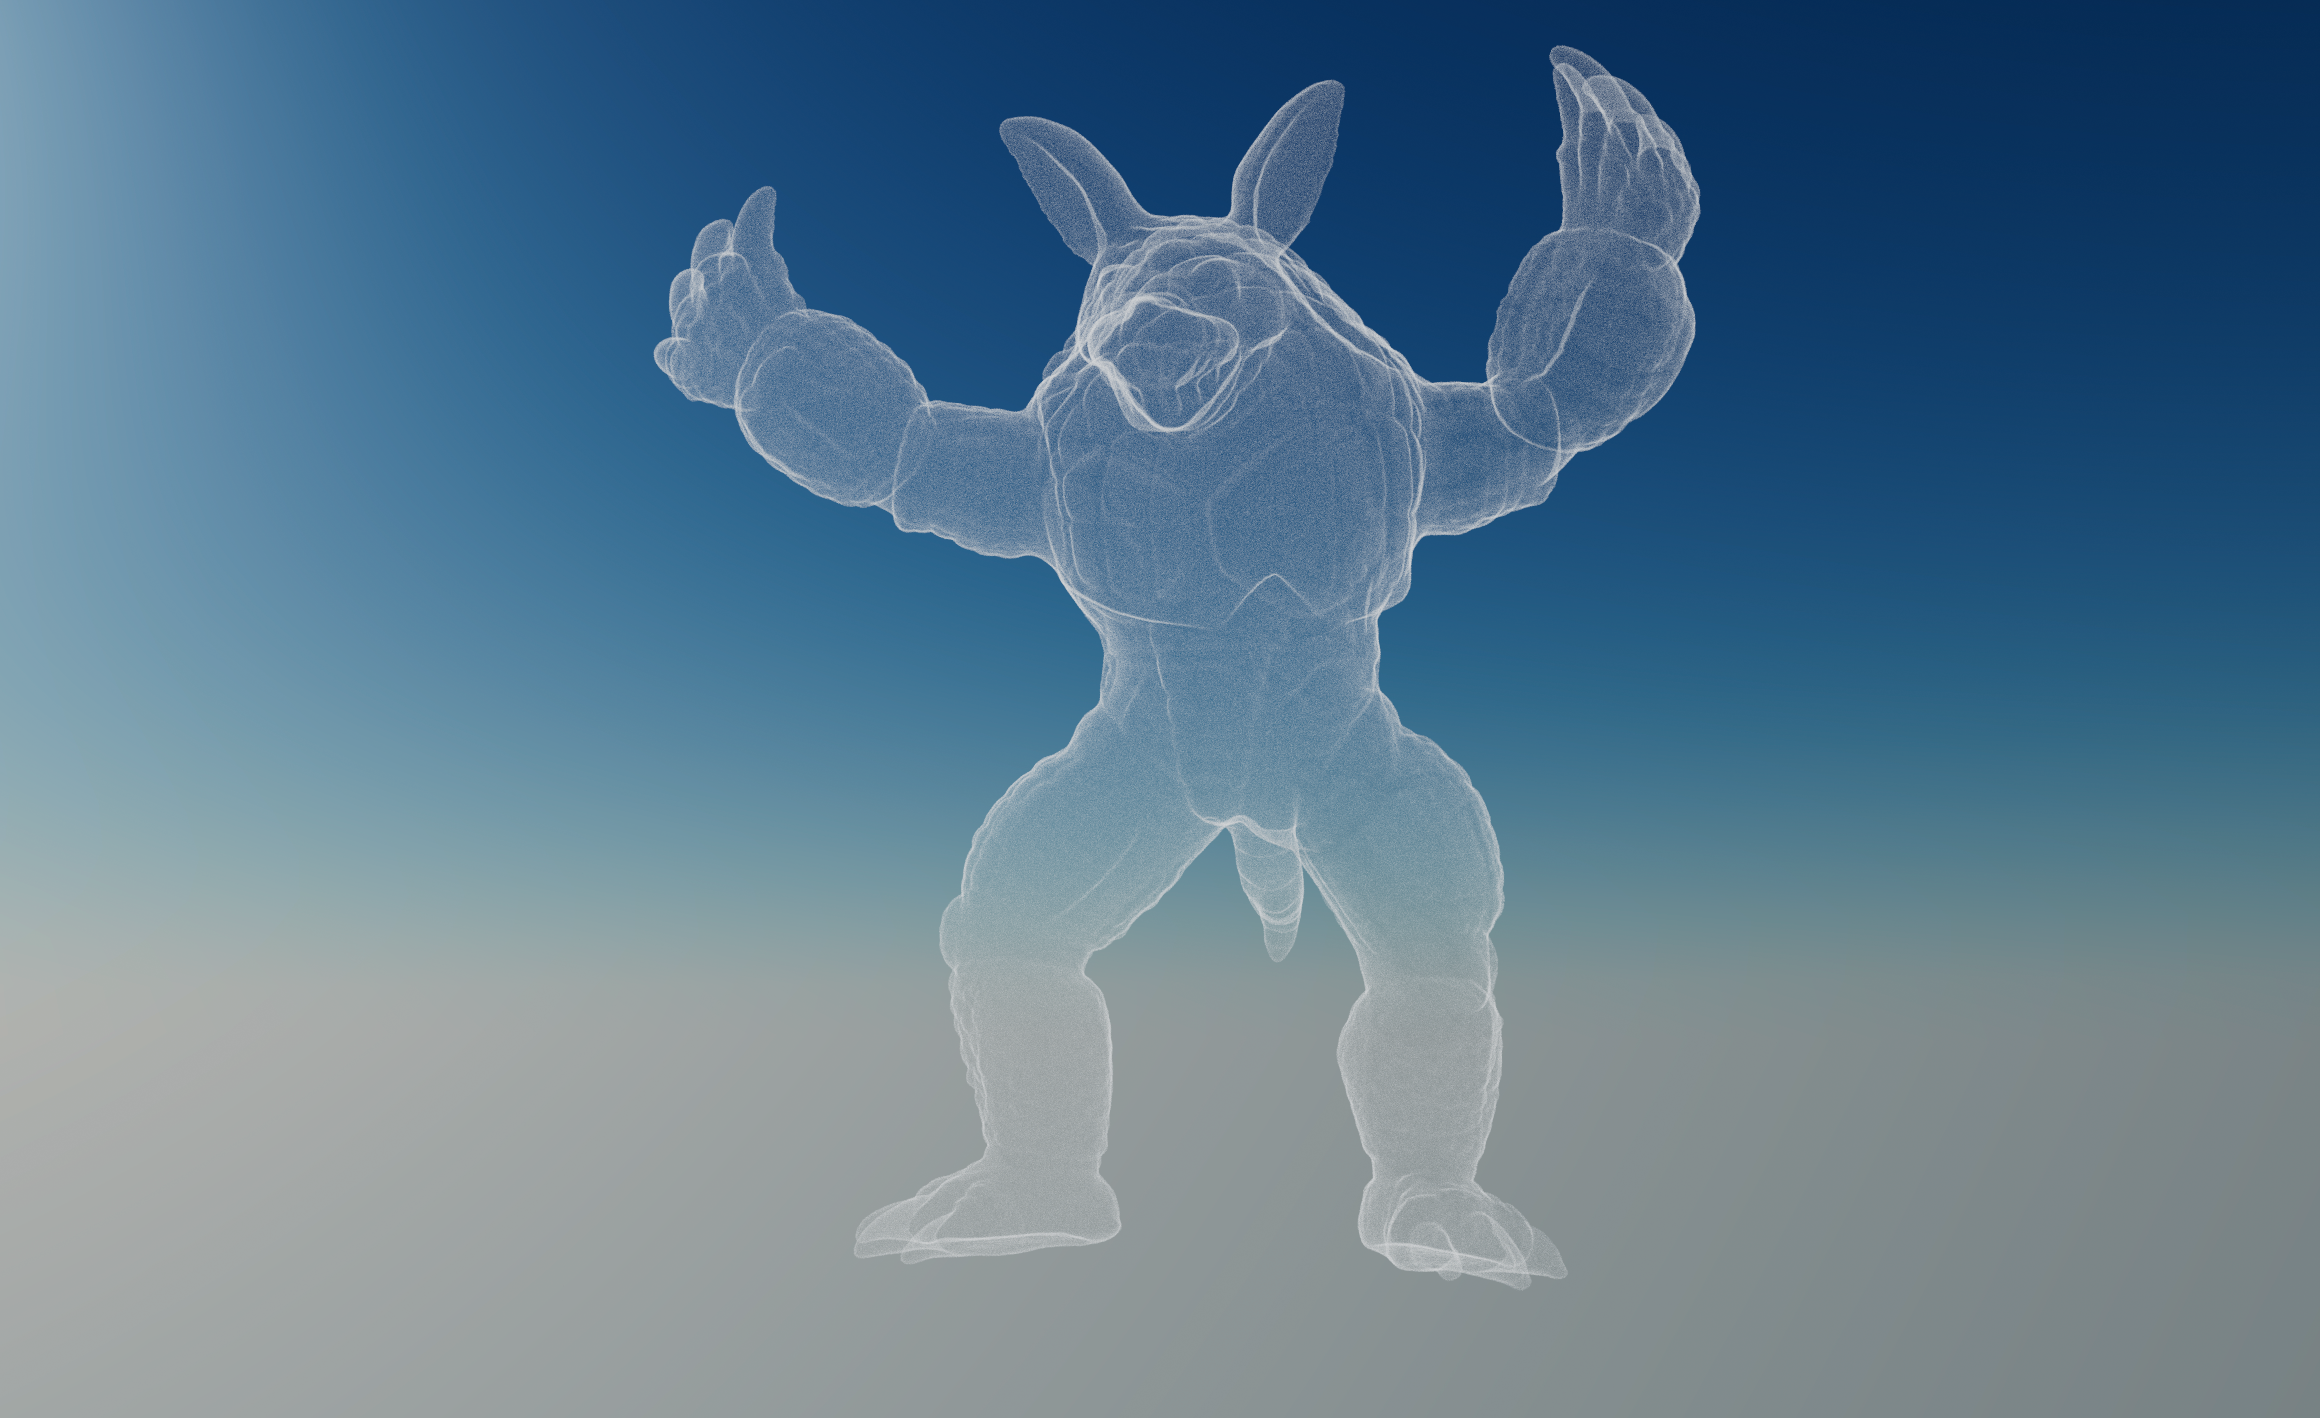
\includegraphics[width=0.3\textwidth]{figures/armadilo.png}
    }
    \hfill
    \subfloat[Dragon]{
        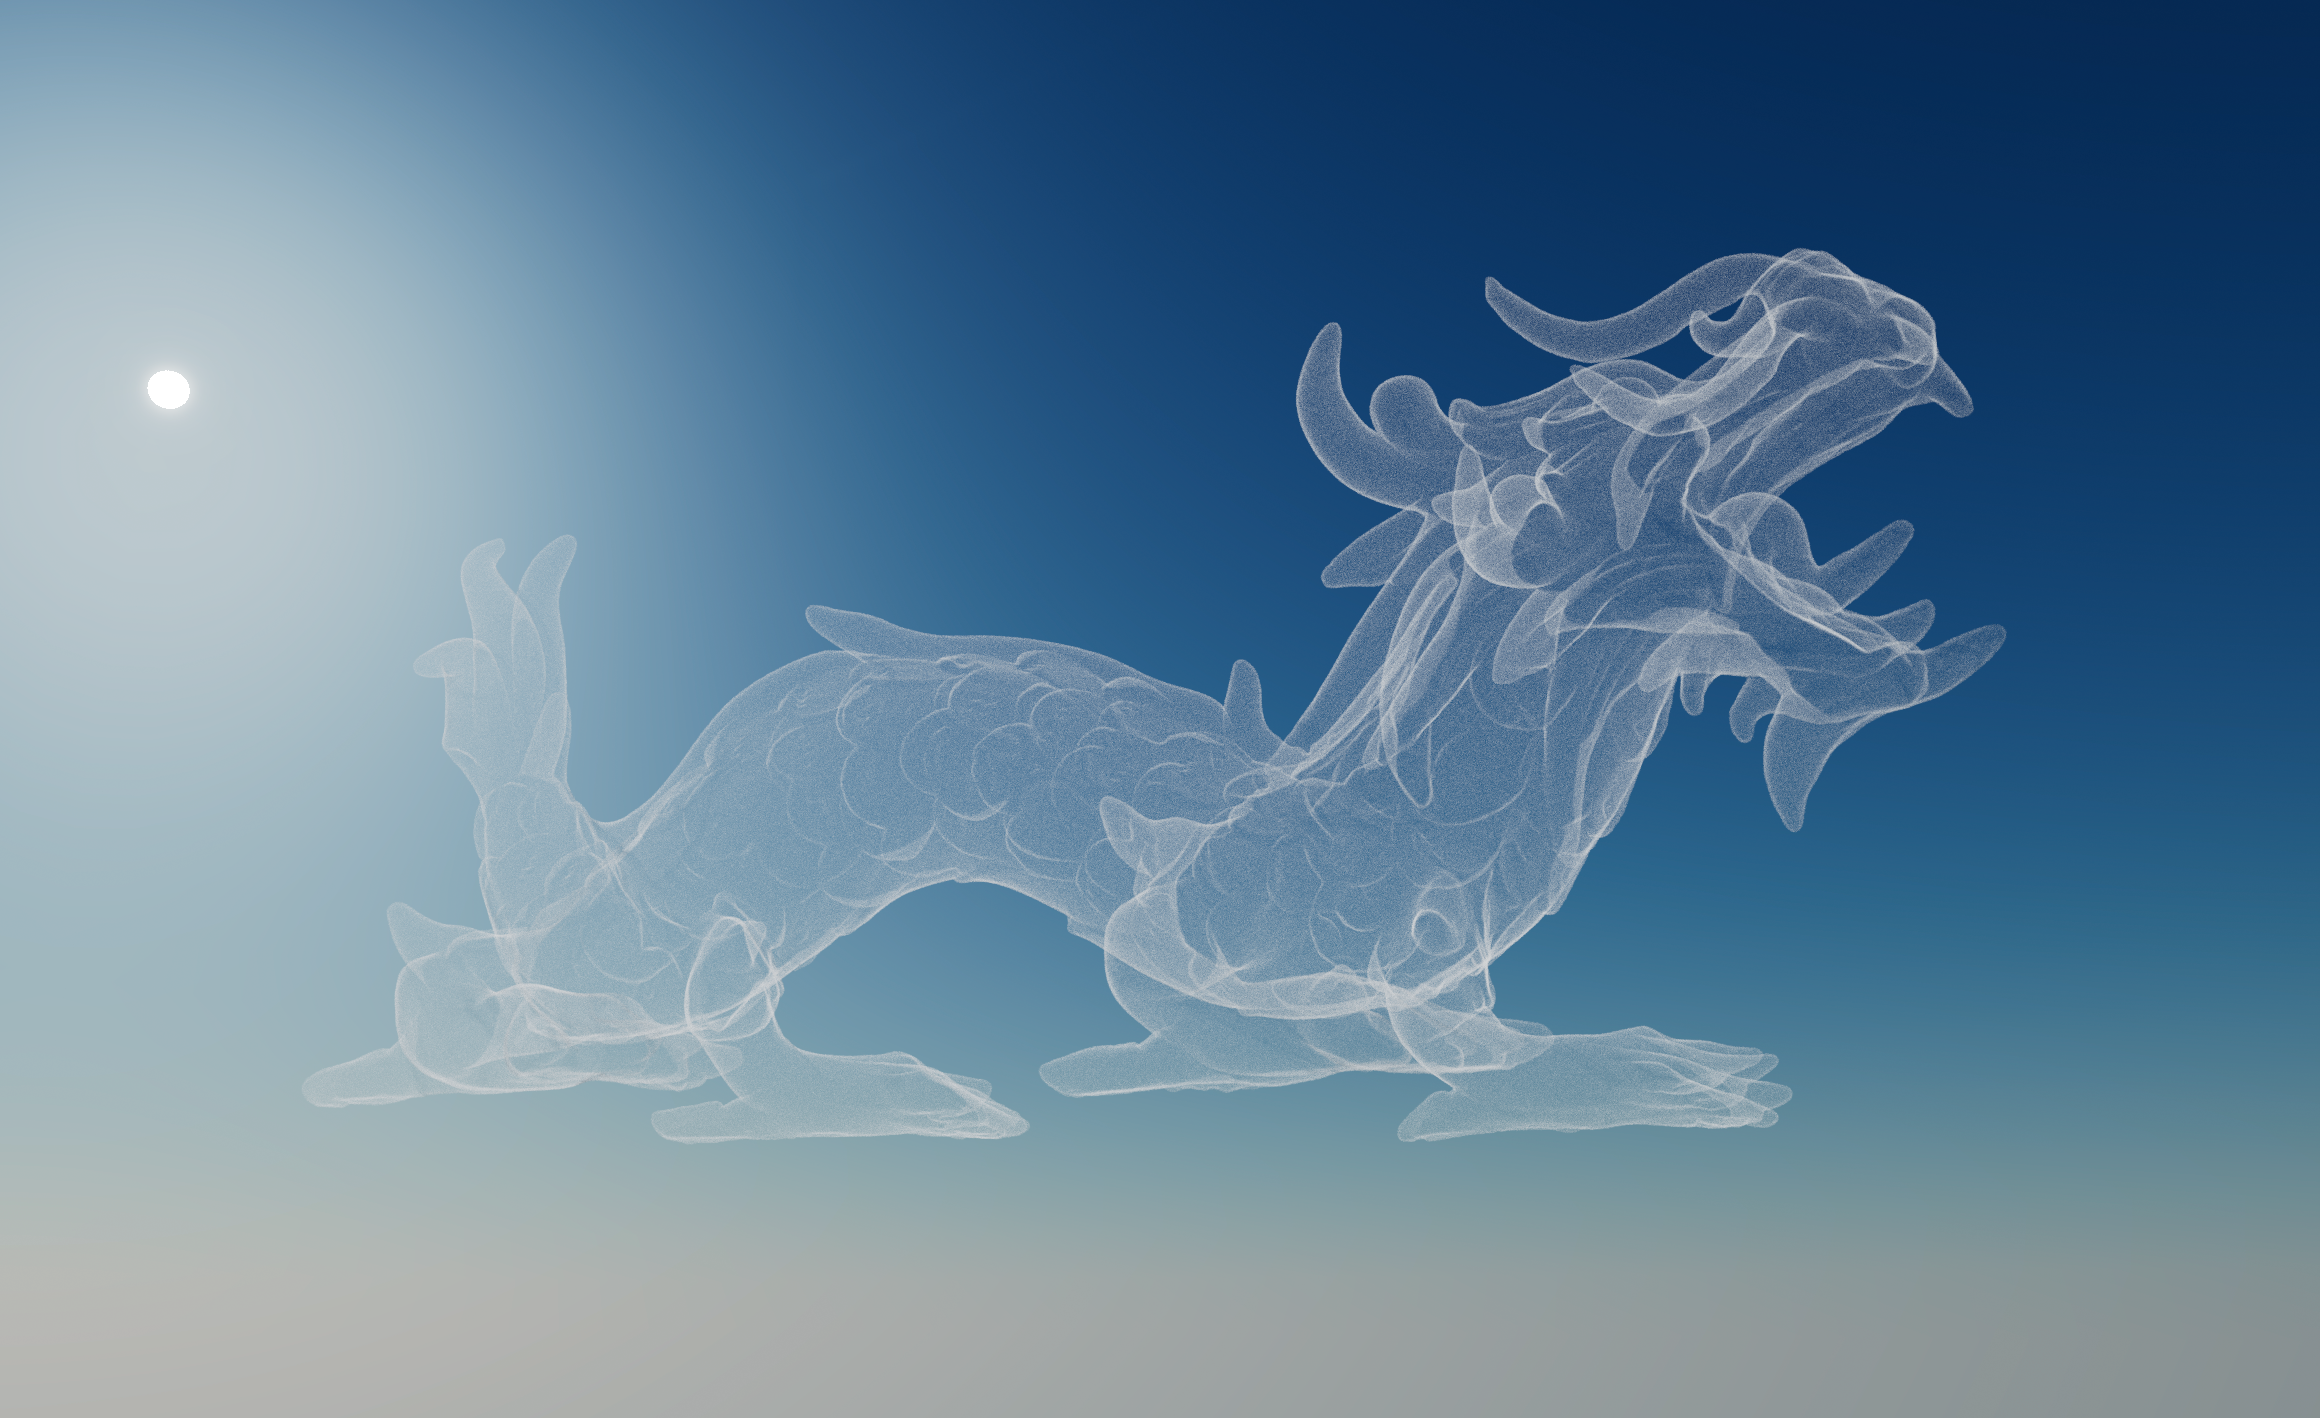
\includegraphics[width=0.3\textwidth]{figures/dragon.png}
    }
    \hfill
    \subfloat[Cloud pack]{
        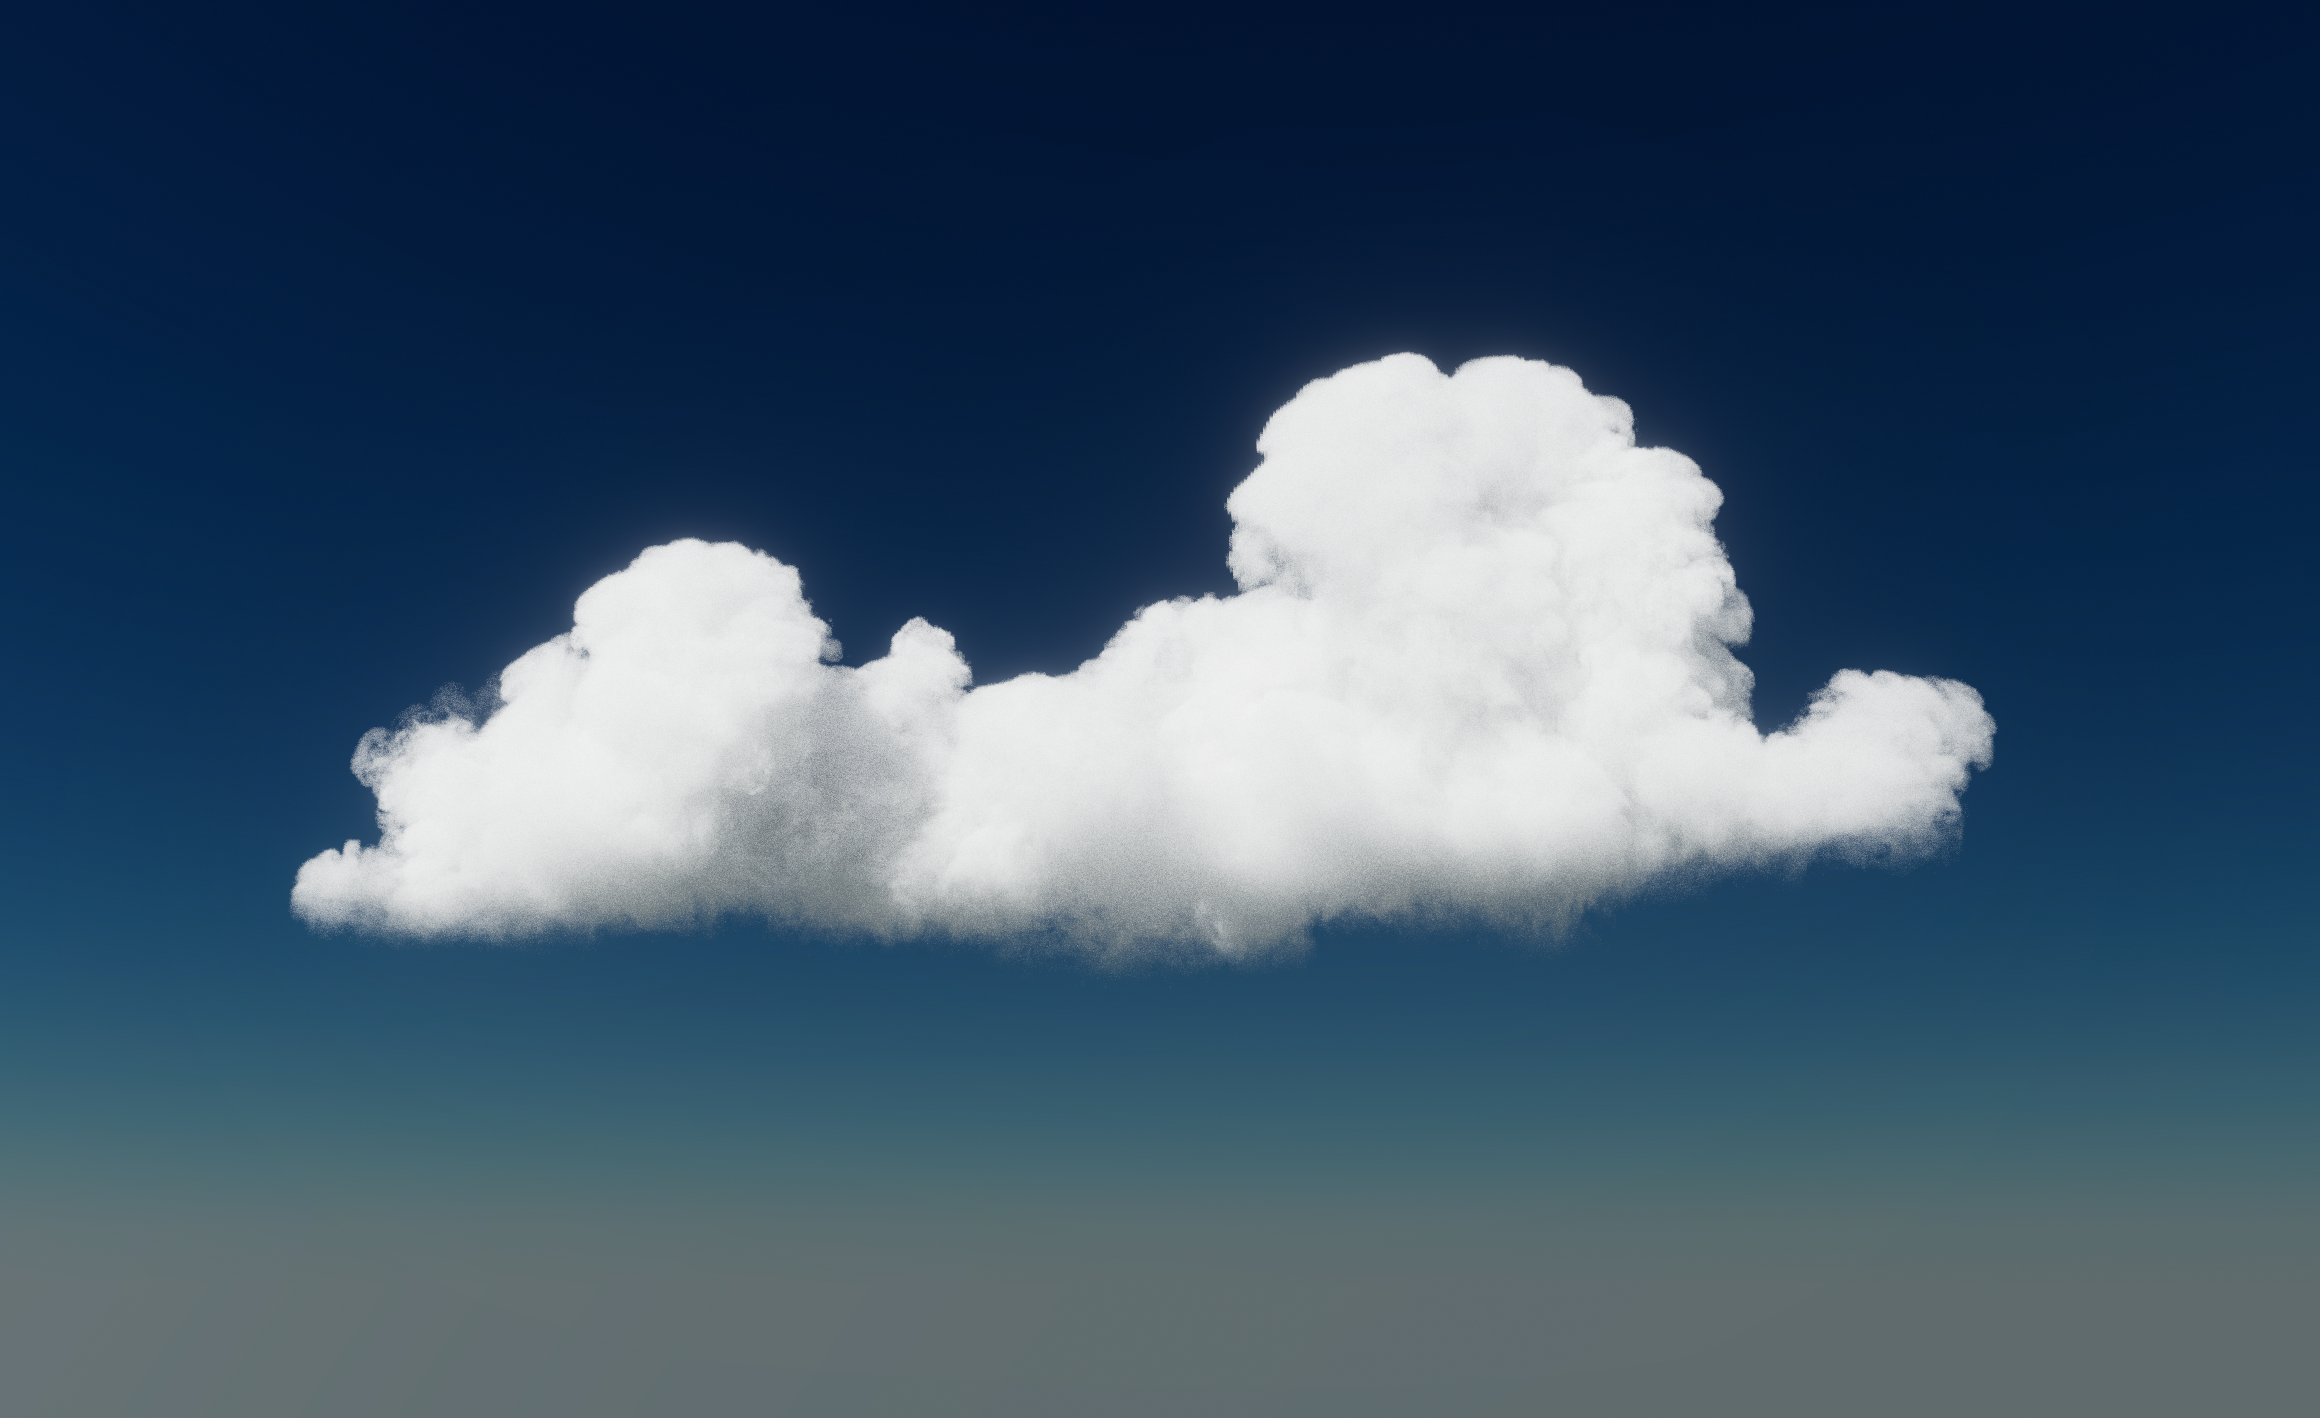
\includegraphics[width=0.3\textwidth]{figures/cloud pack.png}
    }
    \hfill
    \subfloat[Disney Cloud]{
        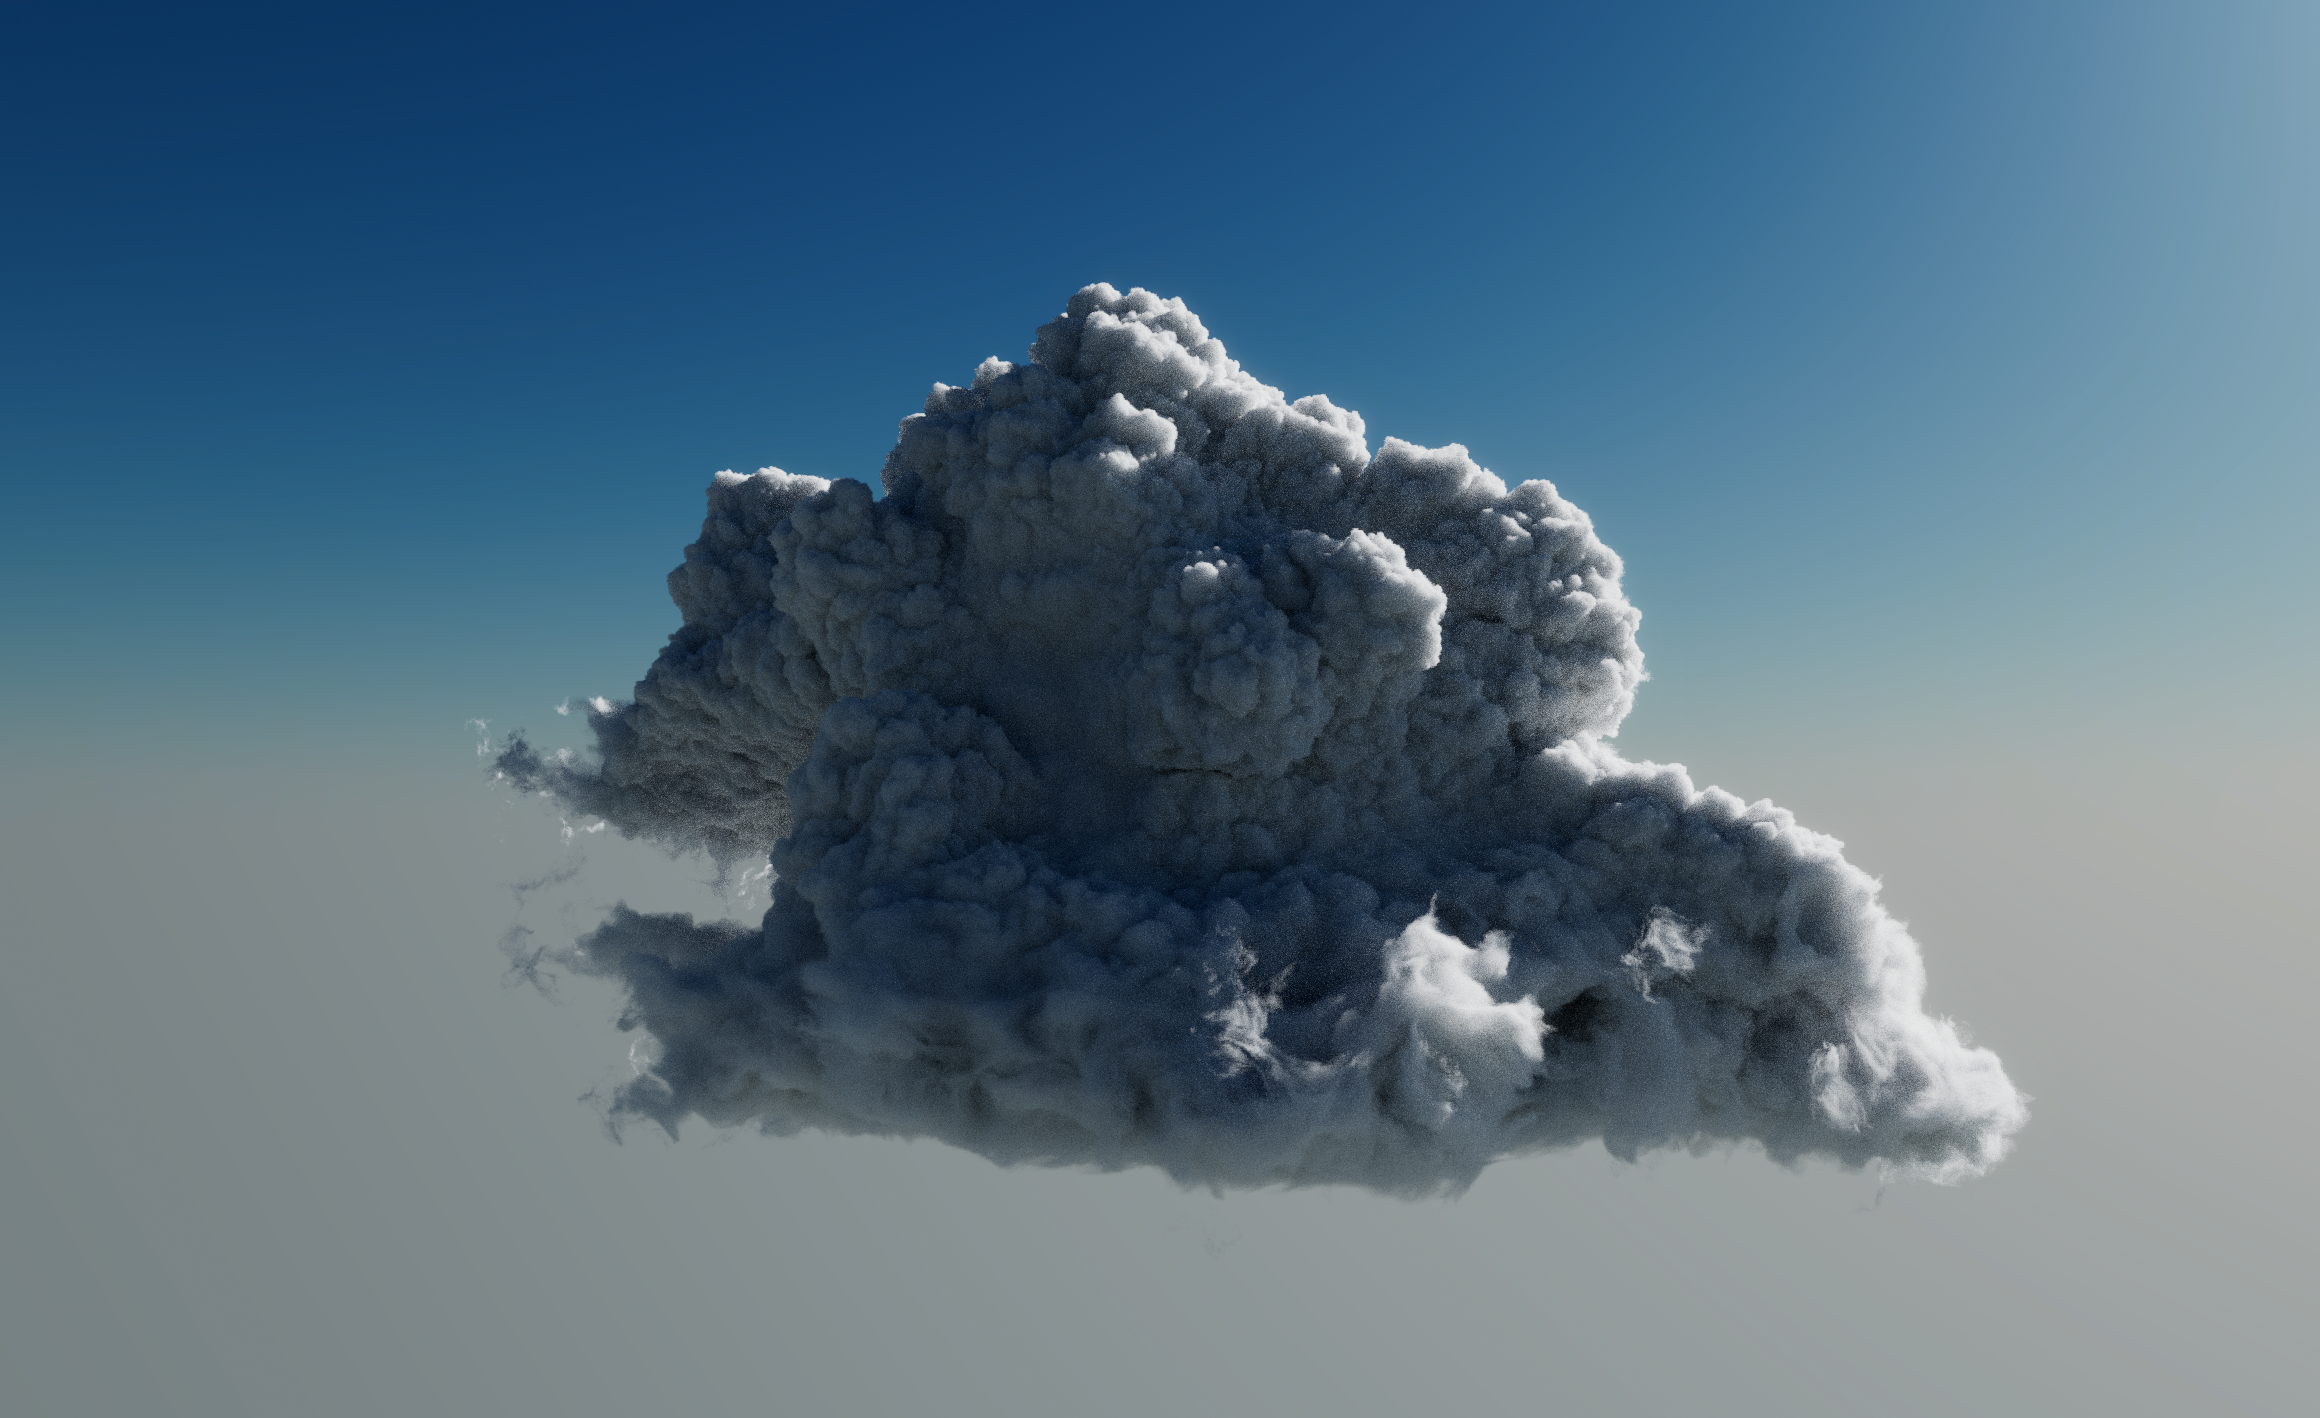
\includegraphics[width=0.3\textwidth]{figures/disney cloud.png}
    }
    \hfill
    \subfloat[Chimney]{
        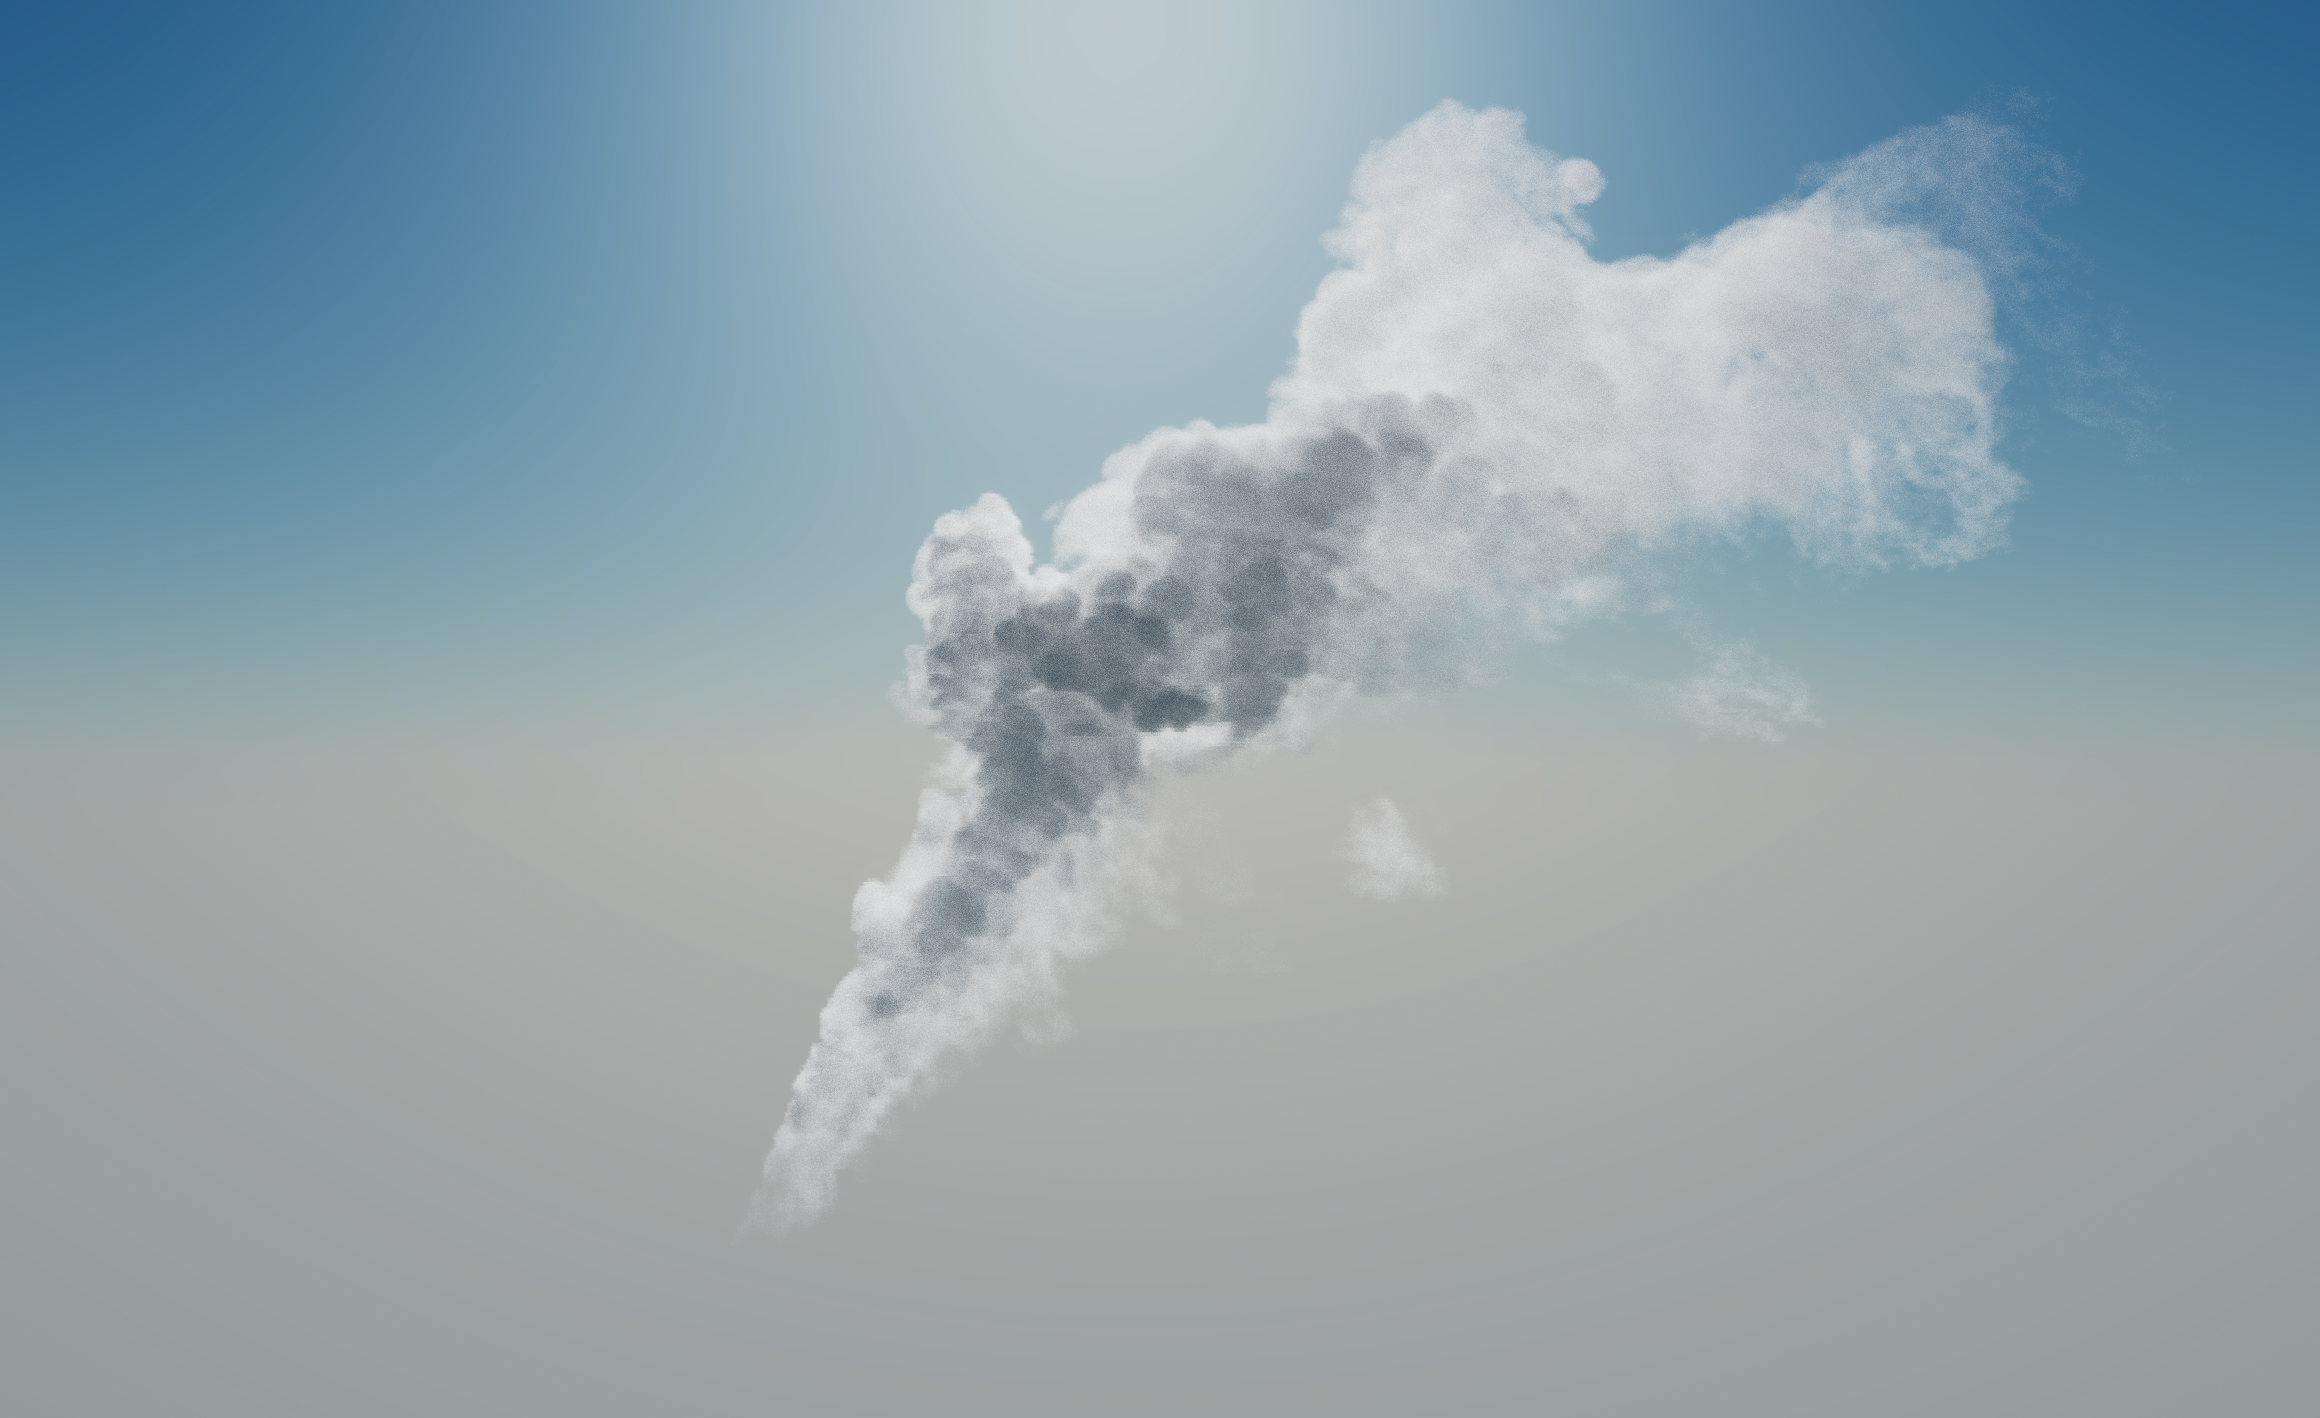
\includegraphics[width=0.3\textwidth]{figures/chimney.png}
    }
    \hfill
    \subfloat[Shockwave]{
        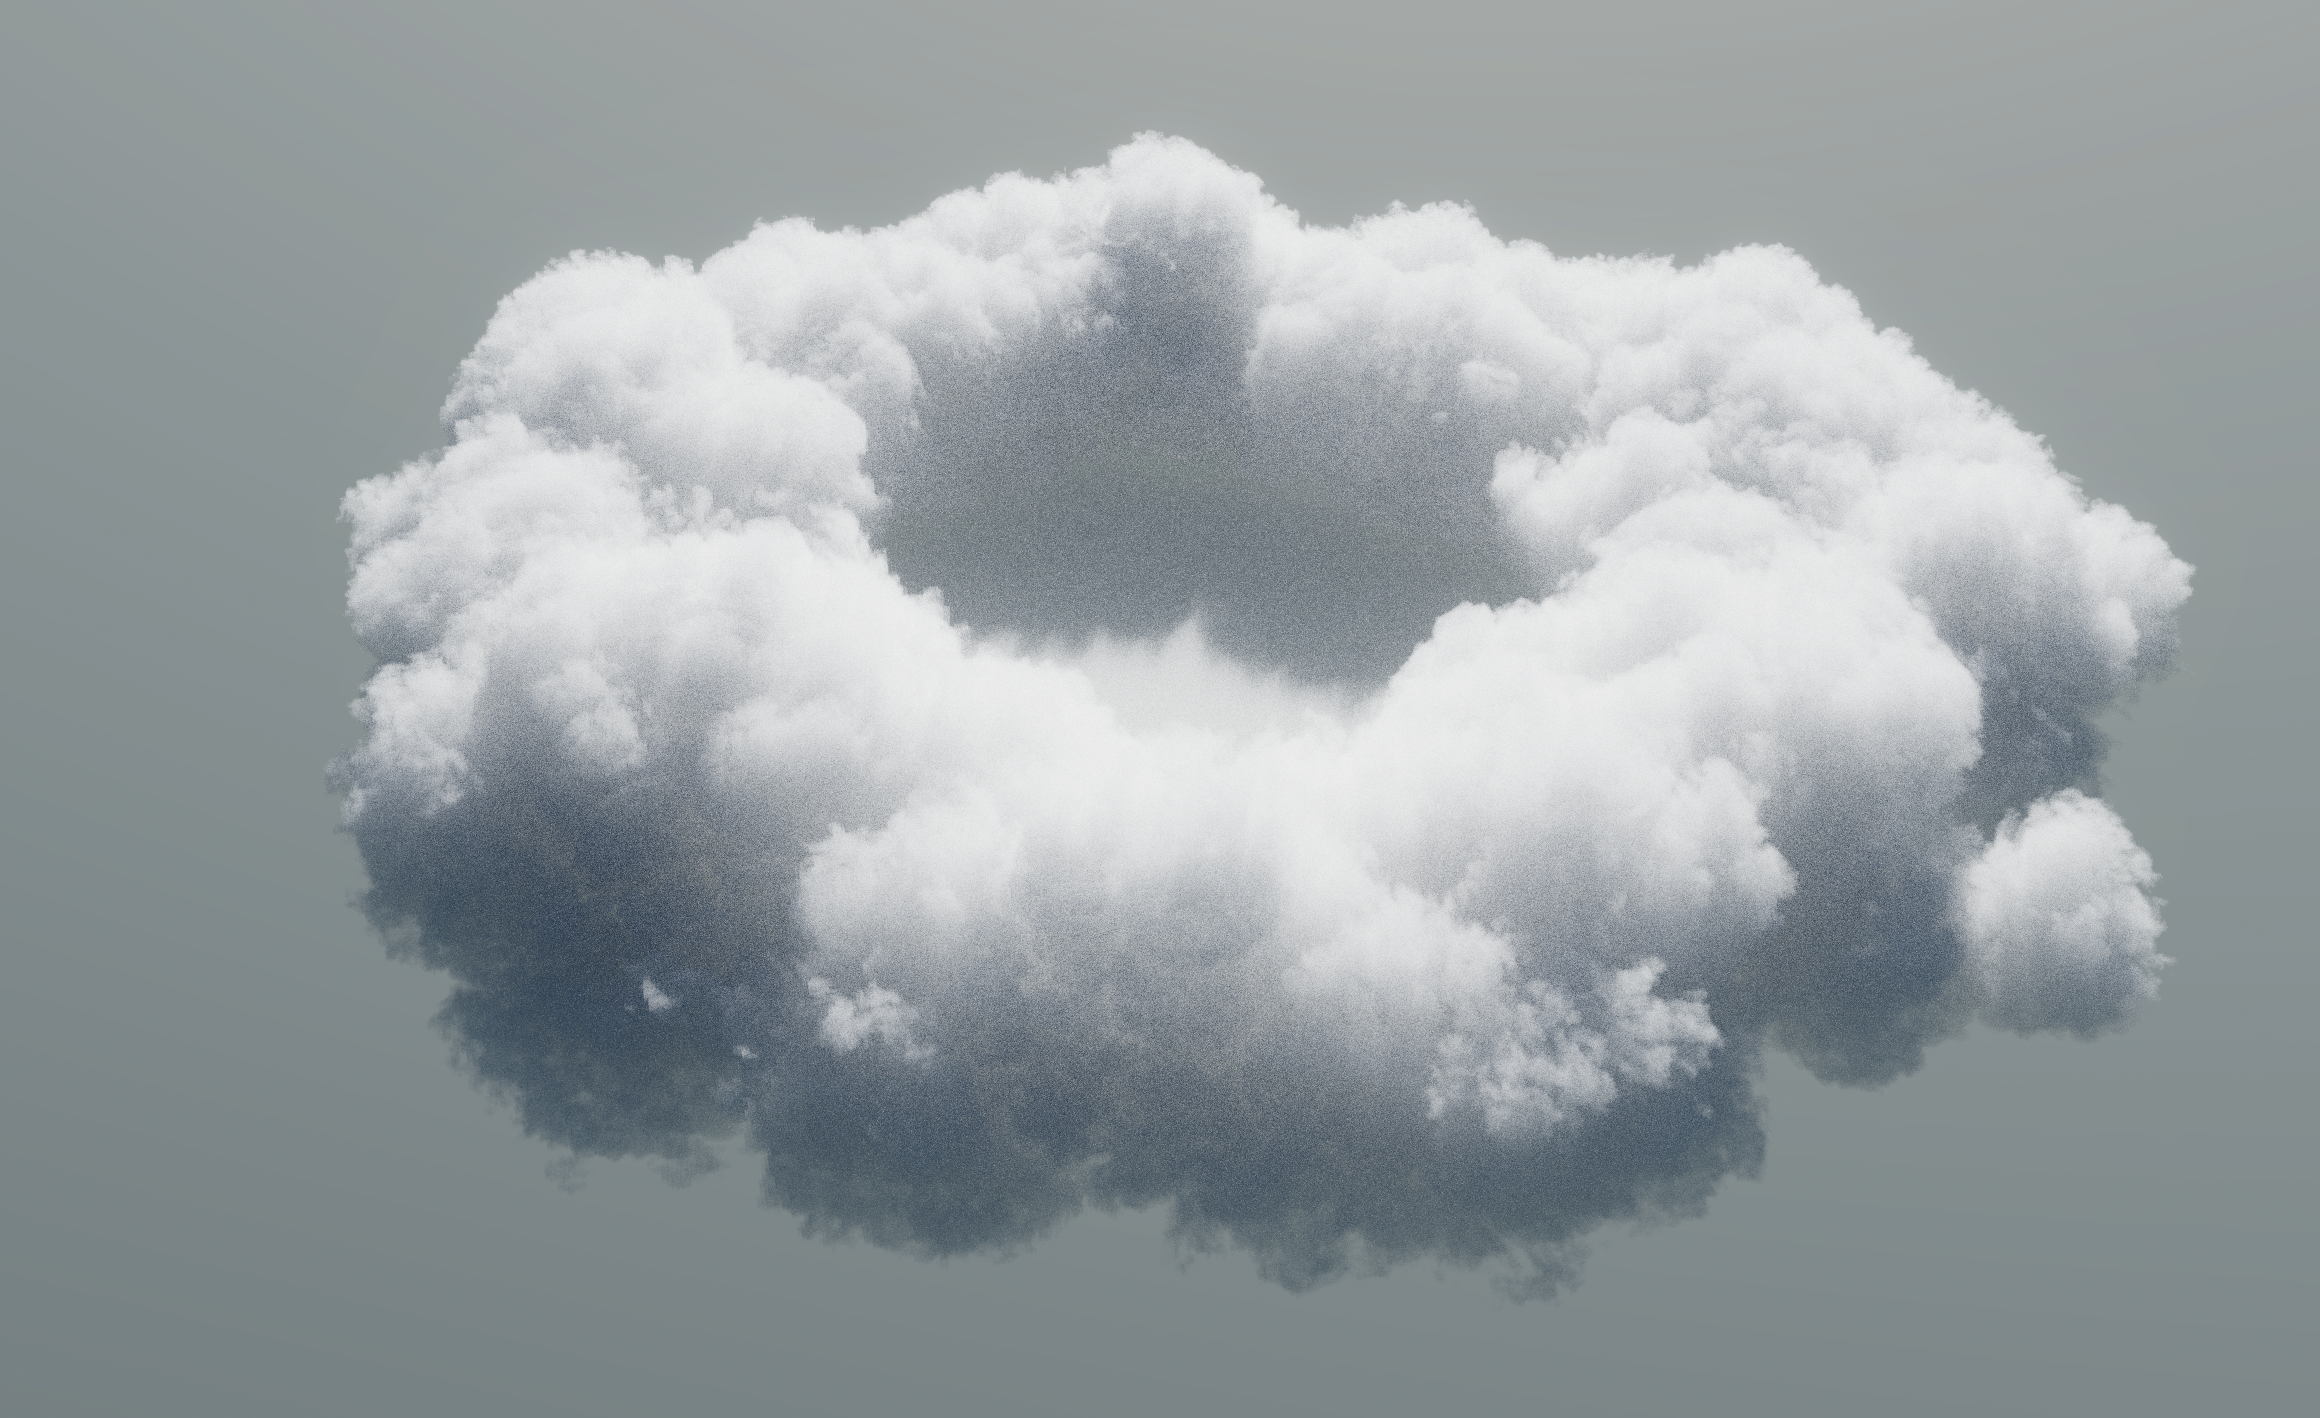
\includegraphics[width=0.3\textwidth]{figures/shockwave.png}
    }
    \hfill
    \subfloat[VDB data]{

        \begin{tabularx}{\textwidth}{|X|c|c|c|c|}
            \hline
            \textbf{Model} & \textbf{Voxels} & \textbf{Dimensions}   & \textbf{Animation frames} \\
            \hline
            Fire           & 4,458,790       & [160, 363, 152]       & 1                         \\
            \hline
            Bunny          & 5,513,993       & [627, 620, 488]       & 1                         \\
            \hline
            Bunny cloud    & 19,210,271      & [576, 571, 437]       & 1                         \\
            \hline
            Armadillo      & 22,734,512      & [1,275, 1,518, 1,159] & 1                         \\
            \hline
            Dragon         & 23,347,893      & [2,022, 910, 1,346]   & 1                         \\
            \hline
            Cloud pack     & 49,869,596      & [349, 178, 530]       & 10                        \\
            \hline
            Disney Cloud   & 188,358,293     & [993, 675, 1,224]     & 1                         \\
            \hline
            Chimney        & 239,747,485     & [160, 350, 505]       & 100                       \\
            \hline
            Shockwave      & 631,494,157     & [732, 140, 729]       & 50                        \\
            \hline
        \end{tabularx}
    }

    \caption{The used volume models for our results. Bunny, armadillo and dragon consist of only the bounding edge of the volume. Cloud pack, chimney and shockwave contain multiple animation frames and thus can make use of delta compression. The voxels column indicates the number of non-zero voxels in the base model. All renders are done using the Breda framework using $100$ samples per pixel. } \label{tab:data-summary}
\end{figure}


\subsection{Tree size} \label{results:tree_size}
In this section we will provide the results of the latter. As described in Section \ref{approach:flipbook_animations}, we put our focus on compressing the voxel data instead of our tree structure size. Because of this, we did not implement any form of compression of the geometry (besides the sparse nature that already existed in VDB). This results in long animation sequences having large trees. In Table \ref{tab:tree_sizes} we can see that the larger models and animation sequences are larger than the in Section \ref{requirements:asset_size} mentioned sizes. This needs to somehow be resolved, either by making our tree deeper or deduplicating bit masks somehow. The latter would be an interesting option. We could make every node in our tree consist of two indices, one child pointer and a bit mask pointer. On one hand, this would add an extra indirection to every level in our tree, but on the other, we will have many internal bit masks where every bit is true. All these nodes will thus point to the same underlying bit mask and pretty much always use cached data. The potential gains here are significant for our L3 nodes, even when all unique bit mask configurations are present. The maximum number of unique L3 nodes is $((1<<3)^3)^2 = 262,144$ which is quite a lot fewer than the number of L3 nodes present in all but one of our models. In the best case, our shockwave model would reduce the size of our L3 nodes by $7\times$, and again, possibly improve performance. In conclusion, the tree sizes for long animation sequences are not very practical currently and are the most notable target for follow-up optimizations.

\begin{table}[htbp]
    \centering
    \begin{tabularx}{\textwidth}{|X|c|c|c|c|c|c|}
        \hline
        \textbf{Model} & \textbf{L1 Nodes} & \textbf{L1 size} & \textbf{L2 Nodes} & \textbf{L2 size} & \textbf{L3 Nodes} & \textbf{L3 size} \\
        \hline
        Fire           & 1                 & 4 KB             & 32,768            & 17 MB            & 65,536            & 4 MB             \\
        \hline
        Bunny          & 1                 & 4 KB             & 32,768            & 17 MB            & 307,200           & 21 MB            \\
        \hline
        Bunny cloud    & 1                 & 4 KB             & 32,768            & 17 MB            & 303,104           & 20 MB            \\
        \hline
        Armadillo      & 1                 & 4 KB             & 32,768            & 17 MB            & 1,339,392         & 91 MB            \\
        \hline
        Dragon         & 1                 & 4 KB             & 32,768            & 17 MB            & 1,302,528         & 88 MB            \\
        \hline
        Cloud pack     & 10                & 41 KB            & 327,680           & 168 MB           & 905,216           & 61 MB            \\
        \hline
        Disney Cloud   & 1                 & 4 KB             & 32,768            & 17 MB            & 1,007,616         & 69 MB            \\
        \hline
        Chimney        & 100               & 410 KB           & 3,276,800         & 1,678 MB         & 9,195,520         & 625 MB           \\
        \hline
        Shockwave      & 50                & 205 KB           & 1,638,400         & 838 MB           & 9,658,368         & 657 MB           \\
        \hline
    \end{tabularx}
    \caption{Tree sizes of the different VDB models. Each node takes exactly one 32-bit index and their bit mask in size. Which makes each L1 node 4100 bytes, each L2 node 516 bytes, and each L3 node 68 bytes. The number of L1 and L2 nodes is directly correlated with the number of animation frames as each frame has a single L1 node, and each of the children of that L1 node is allocated upfront. This makes neither the L1 nor the L2 layer sparse, but the L3 layer is sparse and thus can be smaller than the L2 layer. It's also notable how the trees do not make use of delta compression which adds a fixed cost to every animation frame, making long animations like Chimney very large in memory.}
    \label{tab:tree_sizes}
\end{table}

\subsection{Block compression} \label{results:block_compression}
Block compression theoretically has a good compression ratio, by reducing our voxel data from 32 or 16 bits per voxel to 2. There are two main drawbacks to this method. Those being, (1) the reduced precision arising from the discretization into a single byte. And (2) the spatial dependency of voxel data, meaning that voxels within one brick can become inaccurate if there are outliers. We can single out the first issue by using unsigned normalized bytes (Unorm), interpolated between the minimum and maximum value of the volume. This gives us the same discretization as block compression but without the spatial dependency. For good measure, we also compare against a 16-bit float per voxel version. Most VDBs are already using 16-bit floating point data which will thus not result in any difference between it and the 32-bit version. In Figure \ref{fig:block_compression} we see the difference between the different data formats.

Table \ref{tab:compression_rmse} shows us that all models contain a non-zero RMSE even when using the 16-bit floating point precision (although the precision difference should not be noticeable). This is due to our path tracer being non-deterministic and thus always introducing noise in all kinds of ways. However, this does not have to be an issue when we want to evaluate the accuracy of our lossy compression. Visually there is no difference for any of the models between the 32 and 16-bit formats so, we can take that as a baseline. When we have a look at the bunny and dragon models, we barely see a difference in RMSE when using different formats (the visual difference is rendered in Figure \ref{fig:block_compression:bunny_bc7} and Figure \ref{fig:block_compression:dragon_bc7}). Thus, these models work great with this compression technique. When looking at Disney Cloud we see a spike when going from Unorm to BC7. This is visualized above in Figure \ref{fig:block_compression:disney_unorm} (the Unorm diff) and Figure \ref{fig:block_compression:disney_bc7} (the BC7 diff). Some voxels contain different values compared to their 32-bit counterpart. This likely has to do with quickly varying densities. When having a look at fire we also see a jump in error but this time when going from f16 to Unorm. When having a look at Figure \ref{fig:block_compression:fire_f16} (the f16 diff) and Figure \ref{fig:block_compression:fire_unorm} (the Unorm diff), we see that the problem lies in the top half of the model. Specifically, where the densities are very low. This can be explained by the Unorm discretization not properly capturing the subtle differences in different low-density voxels.

This compression method offers very good compression rates with barely any quality loss in most cases. Only when the model contains many values that are not properly representable, like in Figure \ref{fig:block_compression:disney_unorm}, do we run into significant quality loss.

\subsection{Clustering} \label{results:clustering}
Clustering similar bricks has proven more difficult than simply running k-means on all bricks. The main issue lies in figuring out which bricks contain high-frequency data, and which contain low-frequency data. The former should not be clustered as there is a very low chance that there will be any similar bricks, and thus, reduce the quality if we merge them. In Figure \ref{fig:block_compression_visualized} we see what parameters contribute to a minimized loss of quality with the best compression ratio. As also can be seen in the previously mentioned figure, when bricks with high variance are also being clustered we quickly get blocky volumes, this is not acceptable in Breda. Only in sub-Figure \ref{fig:block_compression_visualized:01} we no longer see blocky regions. A more low-level view of our data can be seen in Figure \ref{fig:implementation:compression:cluster}. Here we see that many similar clusters have been removed and our final voxel data texture contains fewer homogeneous grayscale bricks.  In general, this deduplication method works very well for larger models where many bricks have the potential to be similar. But when models are already small, say less than 50 MB, there is almost nothing to be gained.

\subsection{Ray tracing} \label{results:ray_tracing}
We compare our implementation against the results presented by \cite{NanoVDBBenchmark}. They use an NVIDIA RTX 8000 with 672 GB/s bandwidth and 16.31 Tera floating point operations (TFLOPS), and we use an NVIDIA RTX 3070 TI with 608 GB/s and 21.75 TFLOPS. These numbers do not necessarily indicate performance but do sketch a rough idea of the performance scale.

\begin{figure}[H]
    \centering
    \subfloat[Disney Cloud RMSE between 32-bit float and Unorm formats. We only observe inherent path tracing noise.]{
        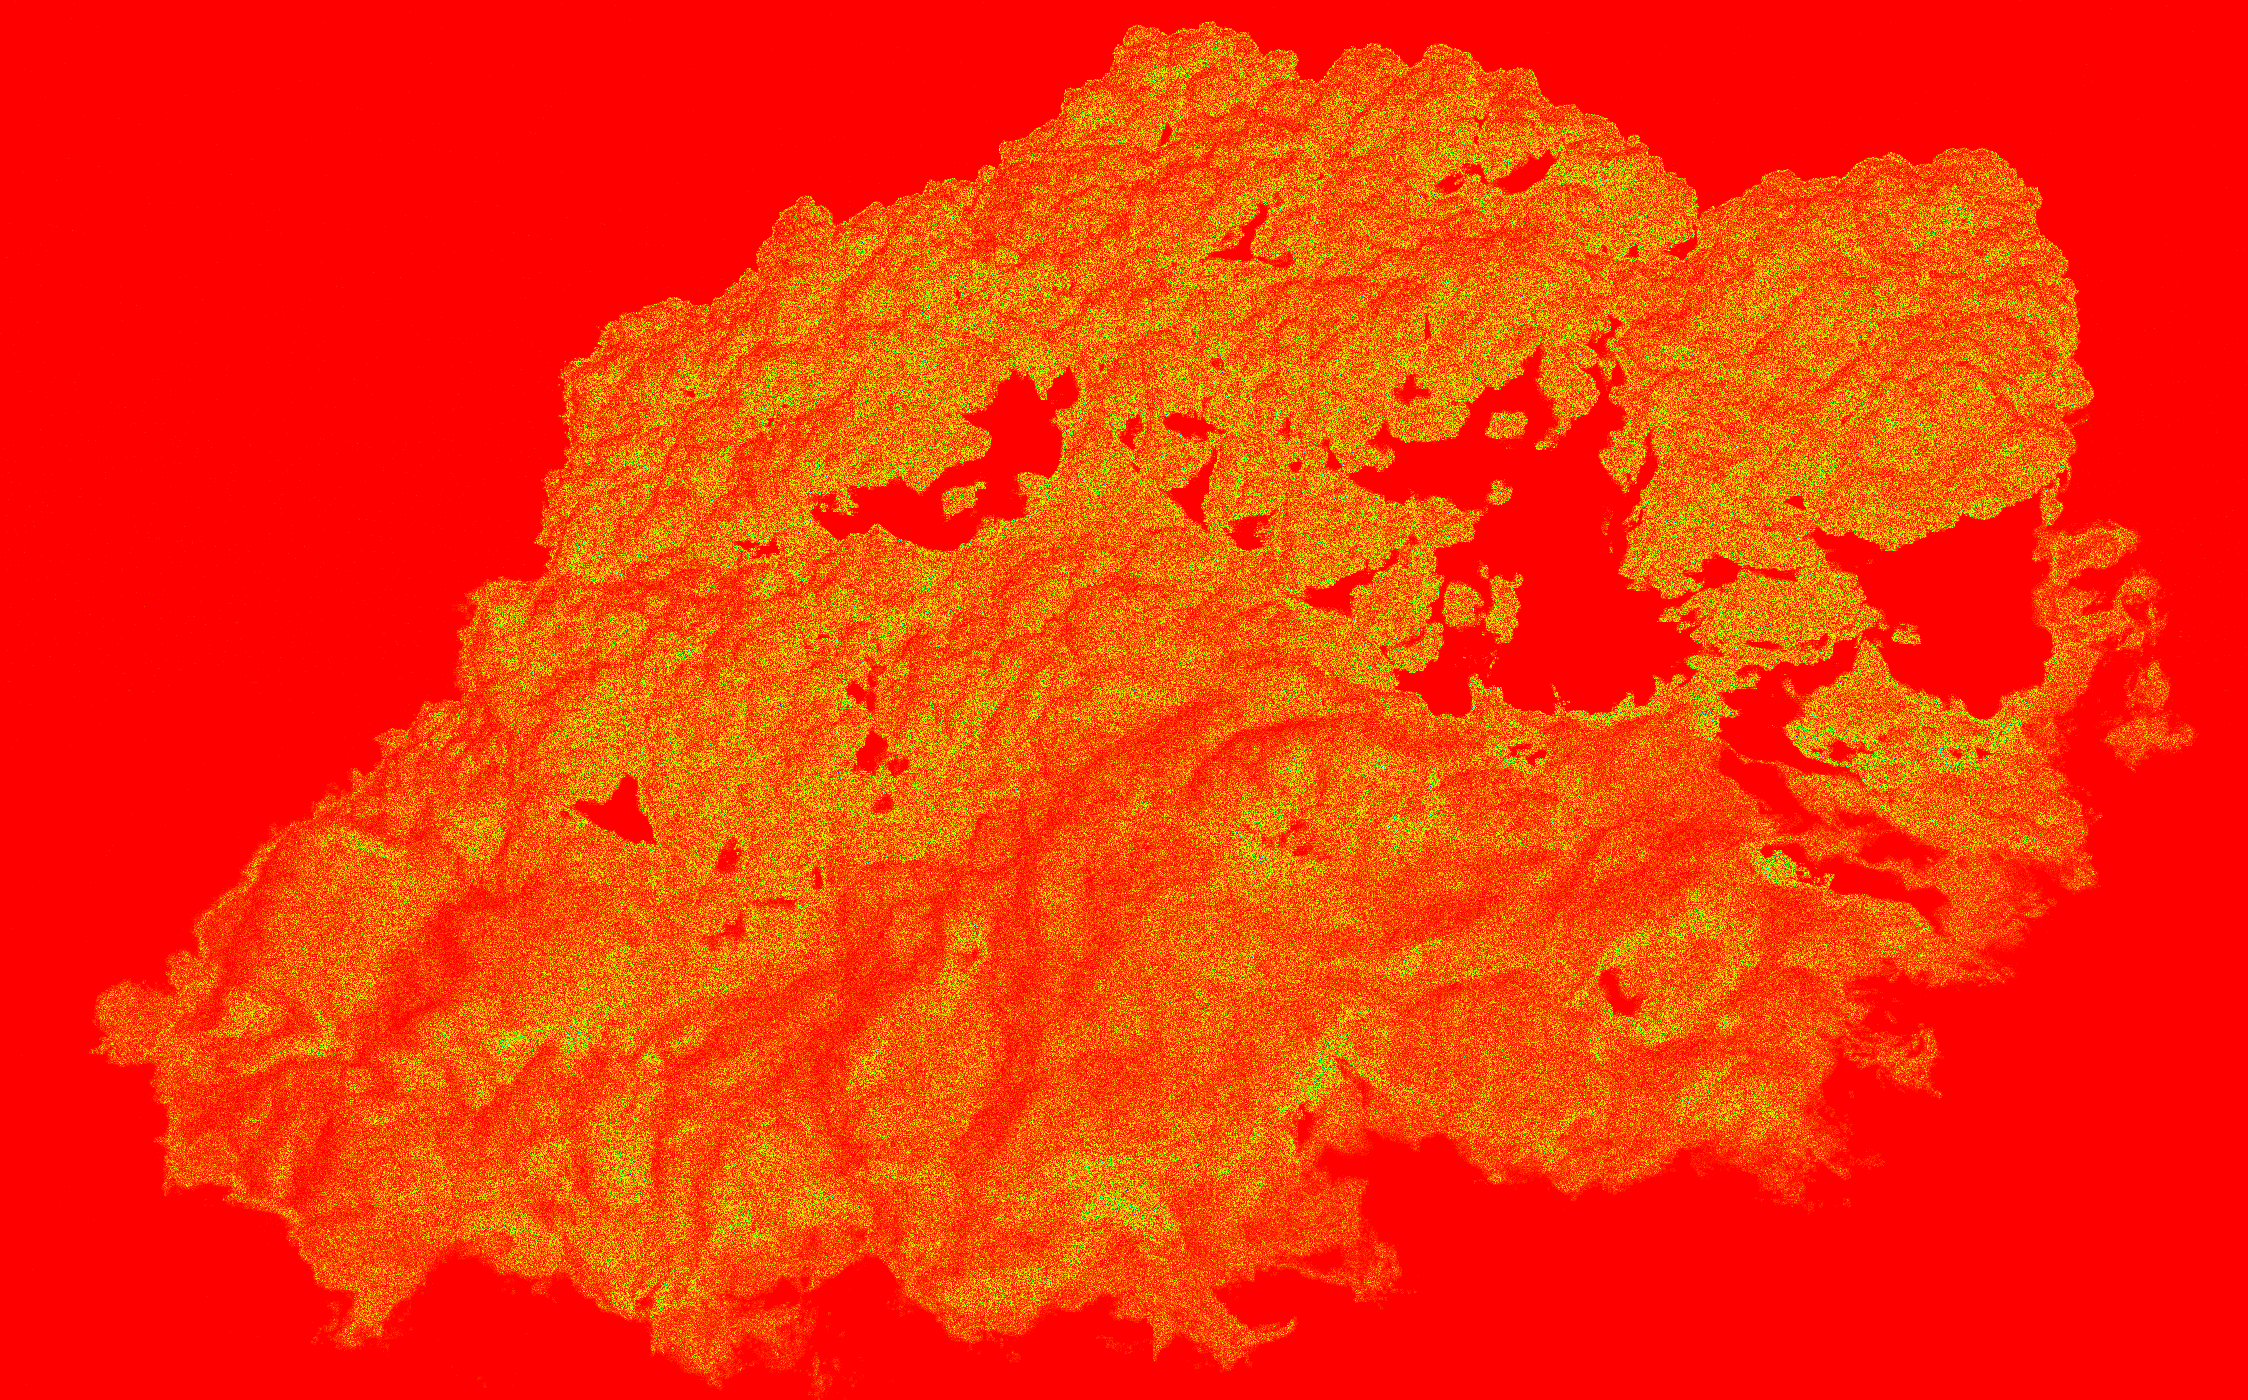
\includegraphics[width=0.3\textwidth]{compare_images_pytorch/diff_disney_cloud_format_unorm.png} \label{fig:block_compression:disney_unorm}
    }
    \hspace{0.2cm}
    \subfloat[Disney Cloud RMSE between 32-bit float and BC7 formats. There is an increase in noise across almost the entire volume, but not in large regions like in Figure \ref{fig:block_compression:fire_unorm}. This tells us that certain voxels in a brick can be wrong, but most of the voxels in each brick are still correct.]{
        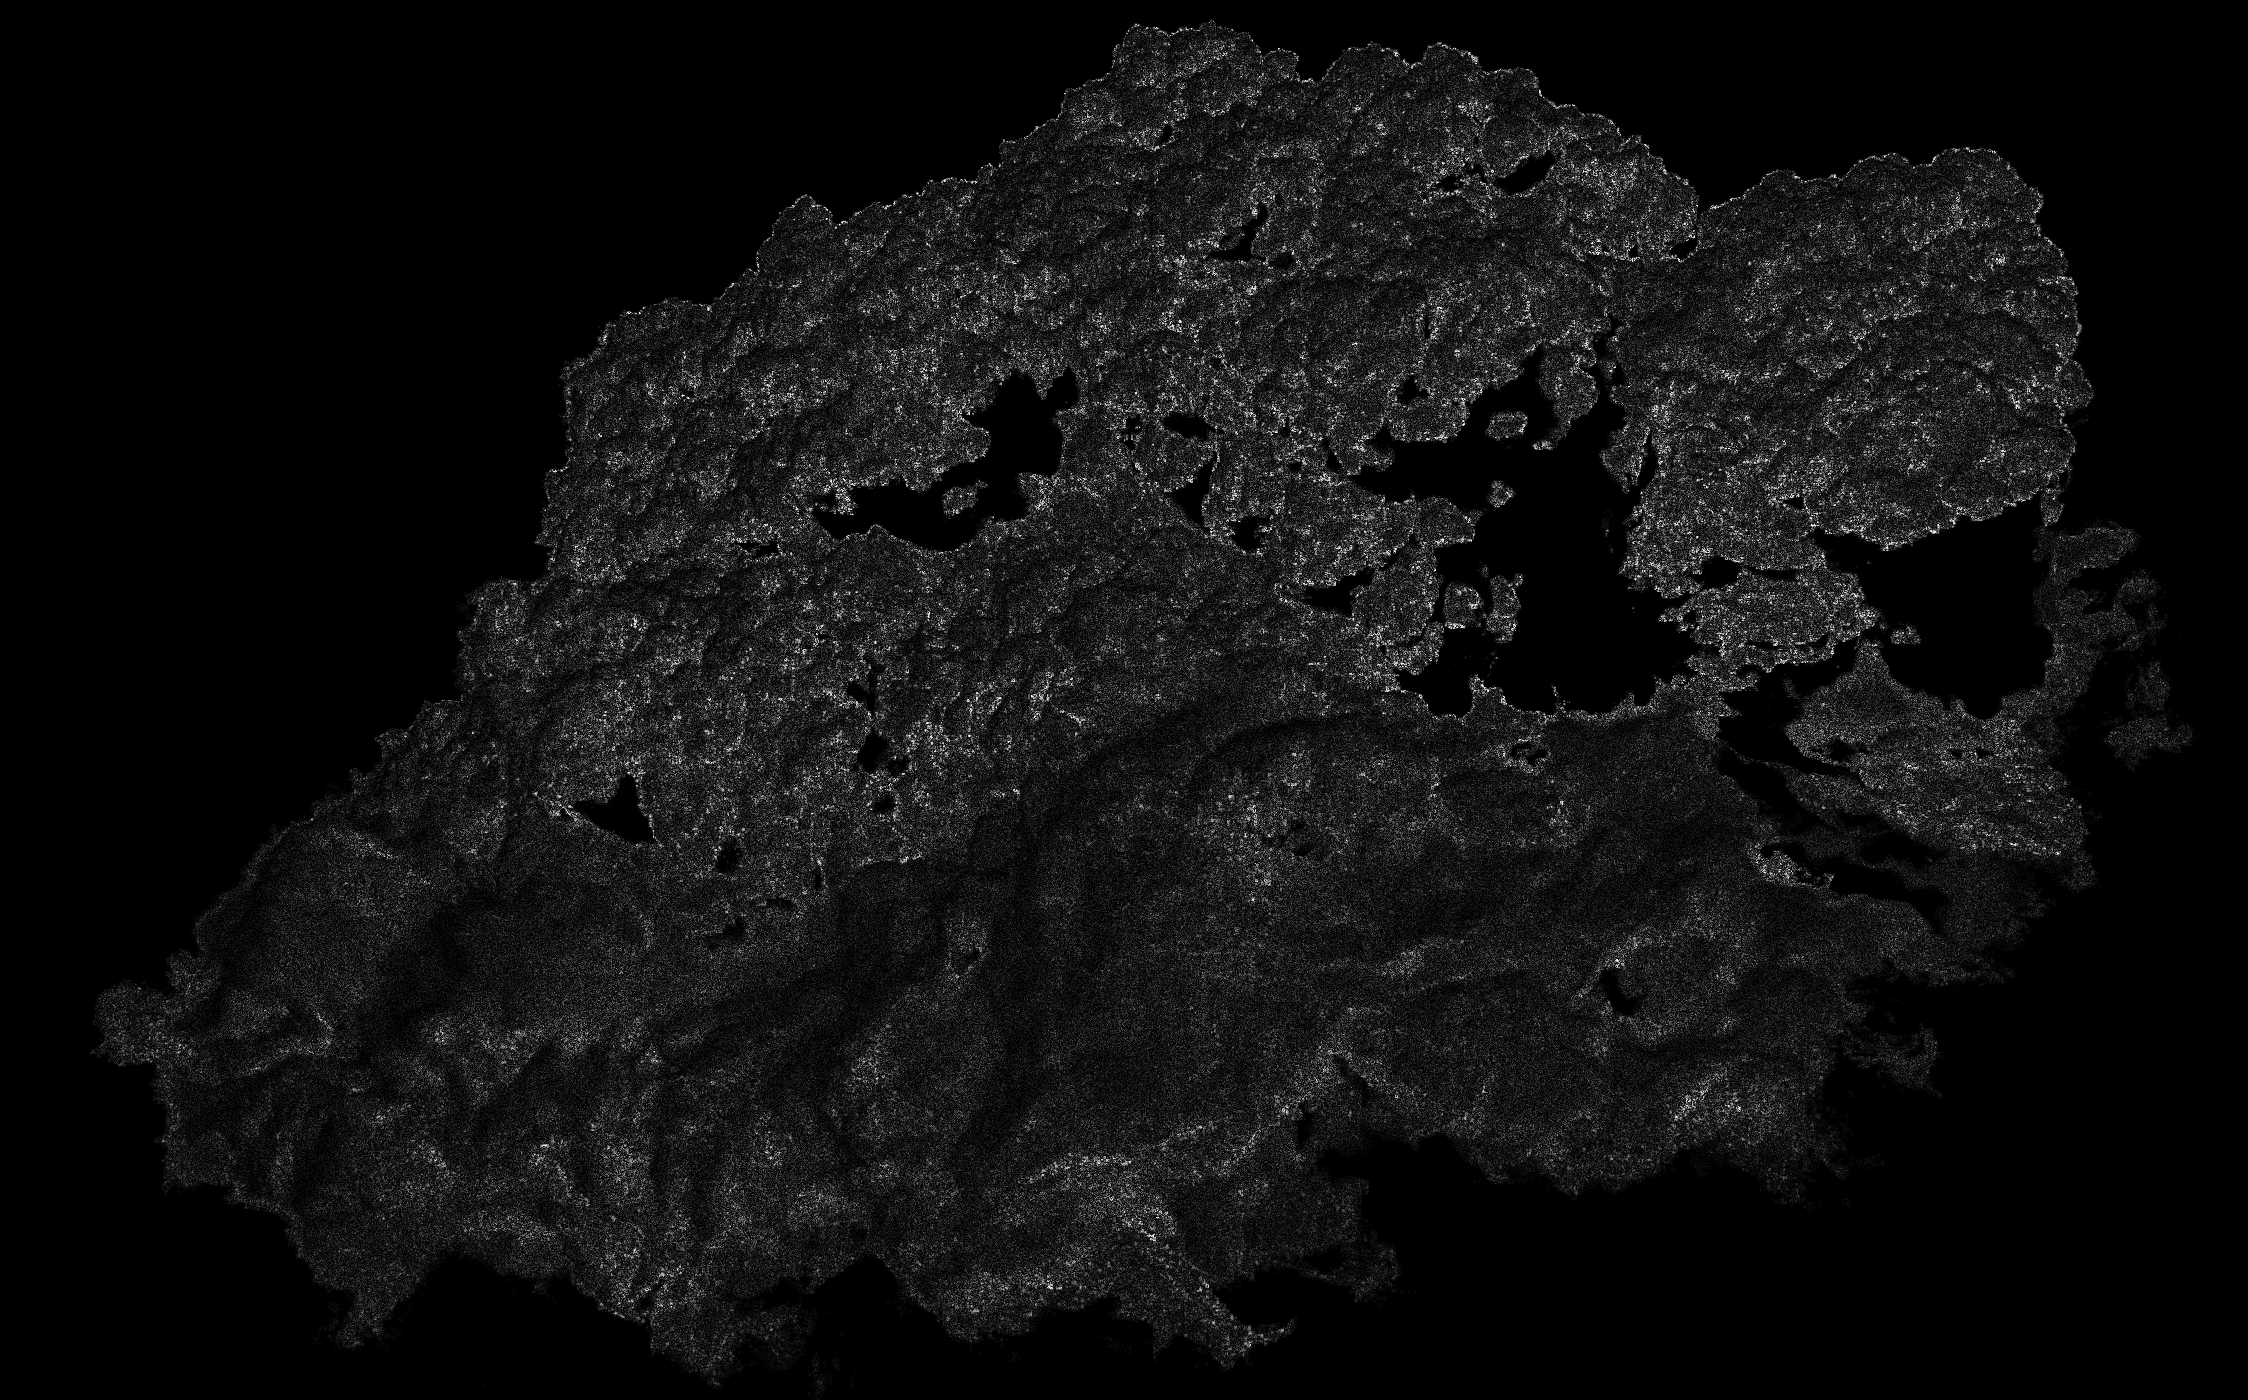
\includegraphics[width=0.3\textwidth]{compare_images_pytorch/diff_disney_cloud_format_bc7.png} \label{fig:block_compression:disney_bc7}
    }
    \hspace{0.2cm}
    \subfloat[Bunny cloud RMSE between 32-bit float and BC7 formats. We only observe inherent path tracing noise.]{
        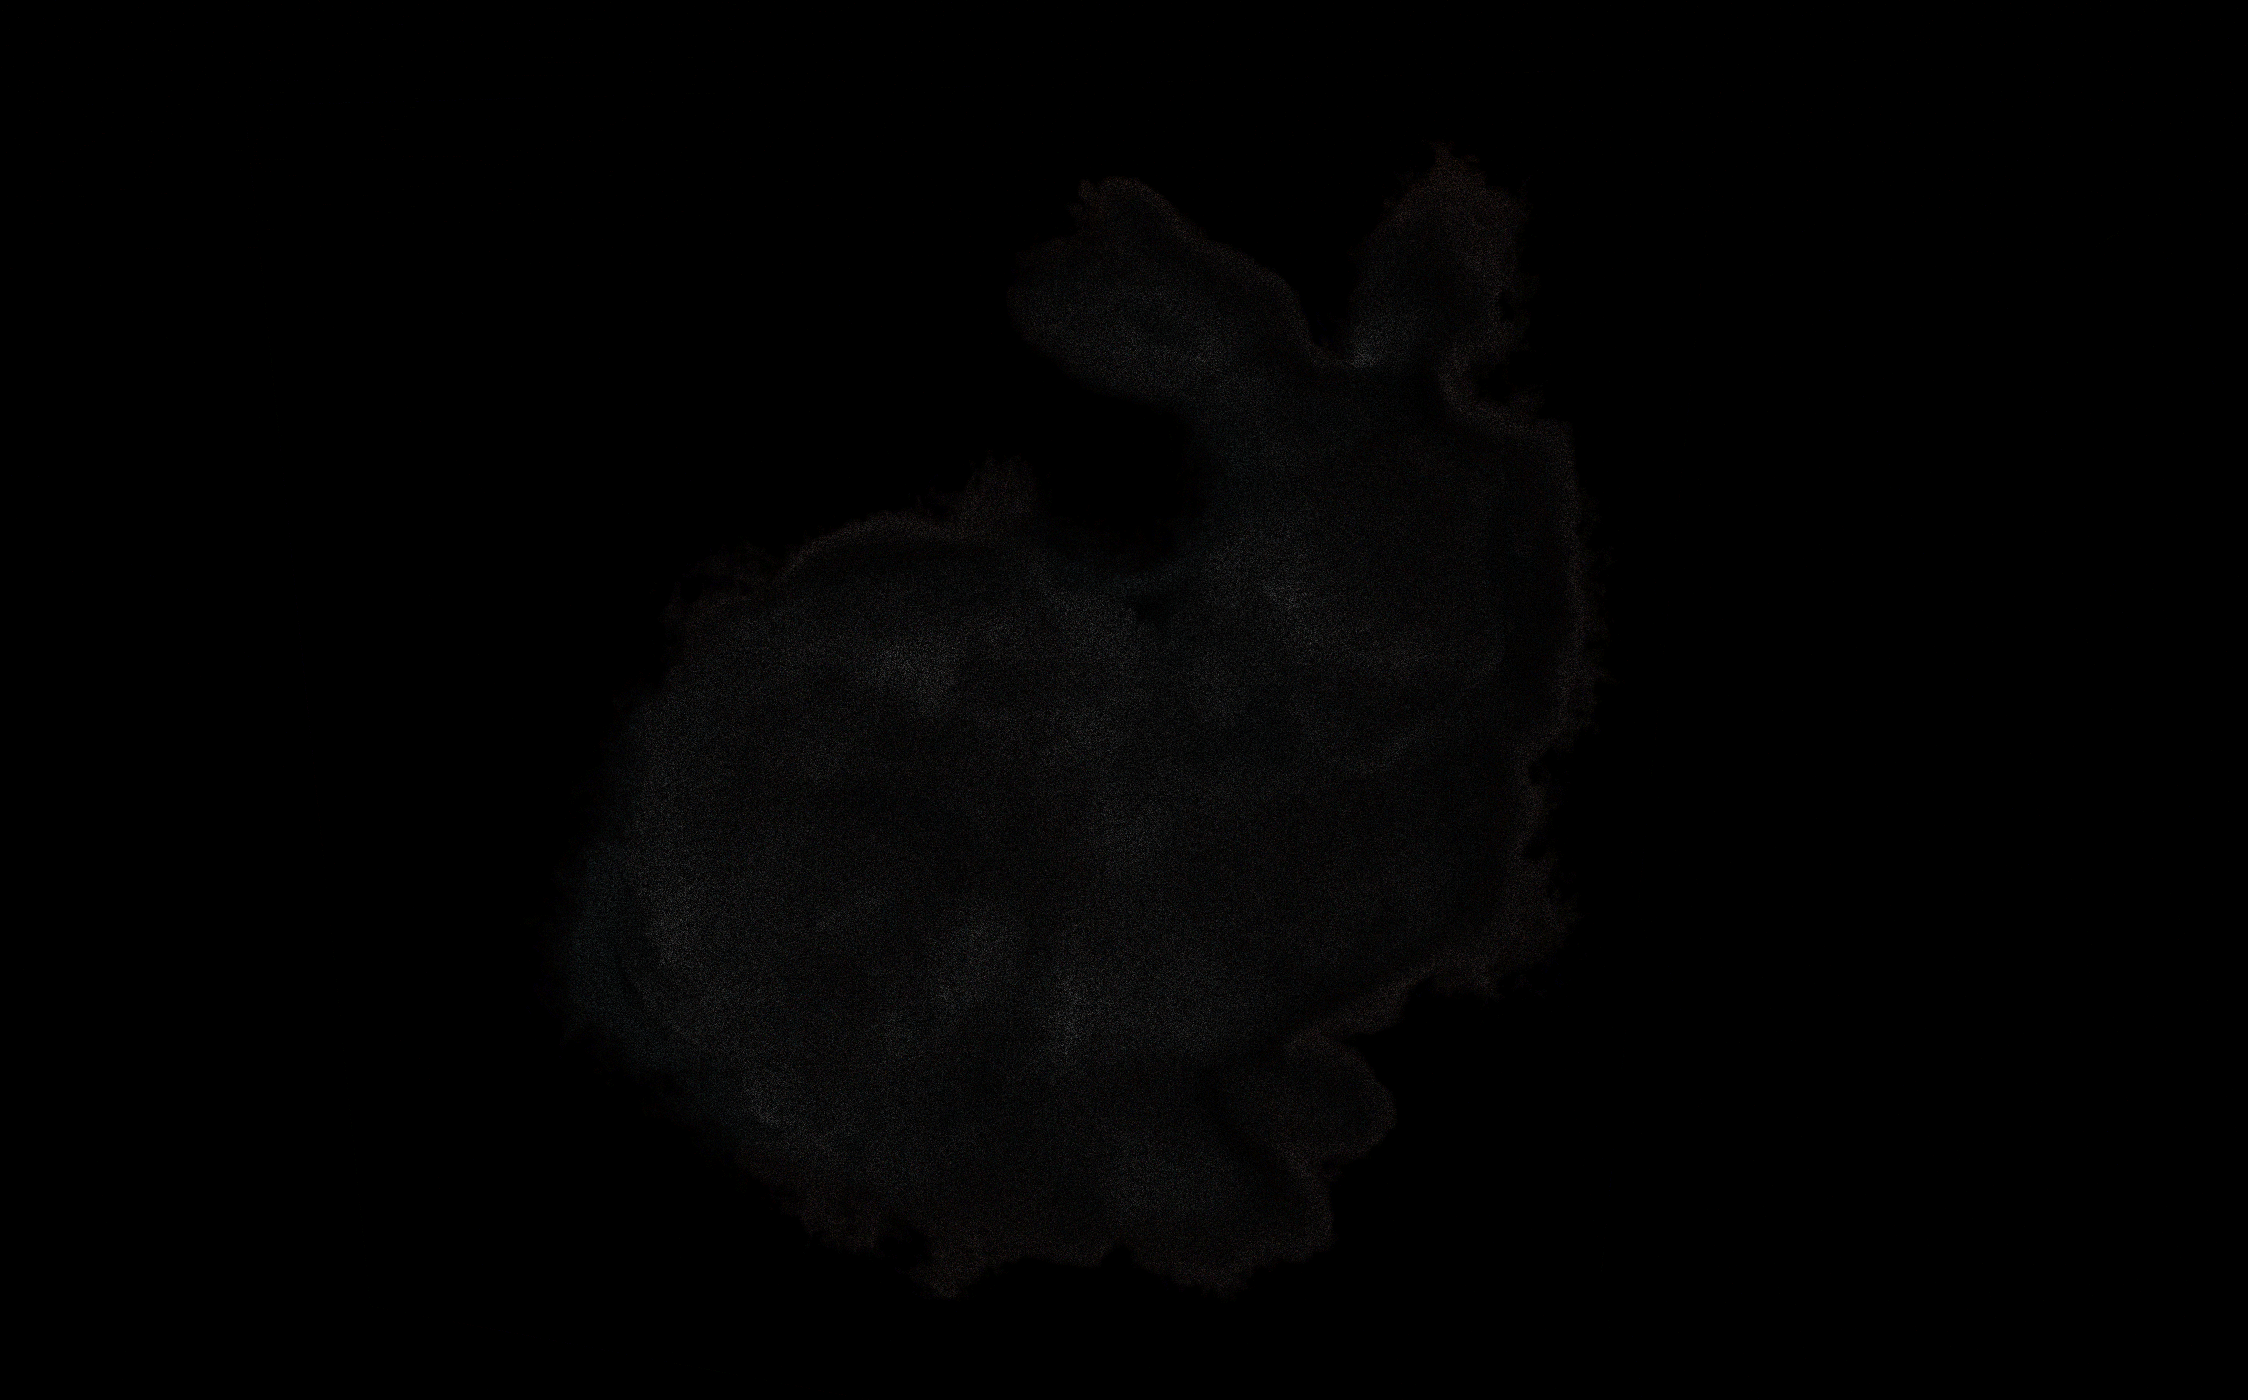
\includegraphics[width=0.3\textwidth]{compare_images_pytorch/diff_bunny_format_bc7.png} \label{fig:block_compression:bunny_bc7}
    }
    \hfill
    \subfloat[Fire RMSE between 32-bit float and f16. We only observe inherent path tracing noise.]{
        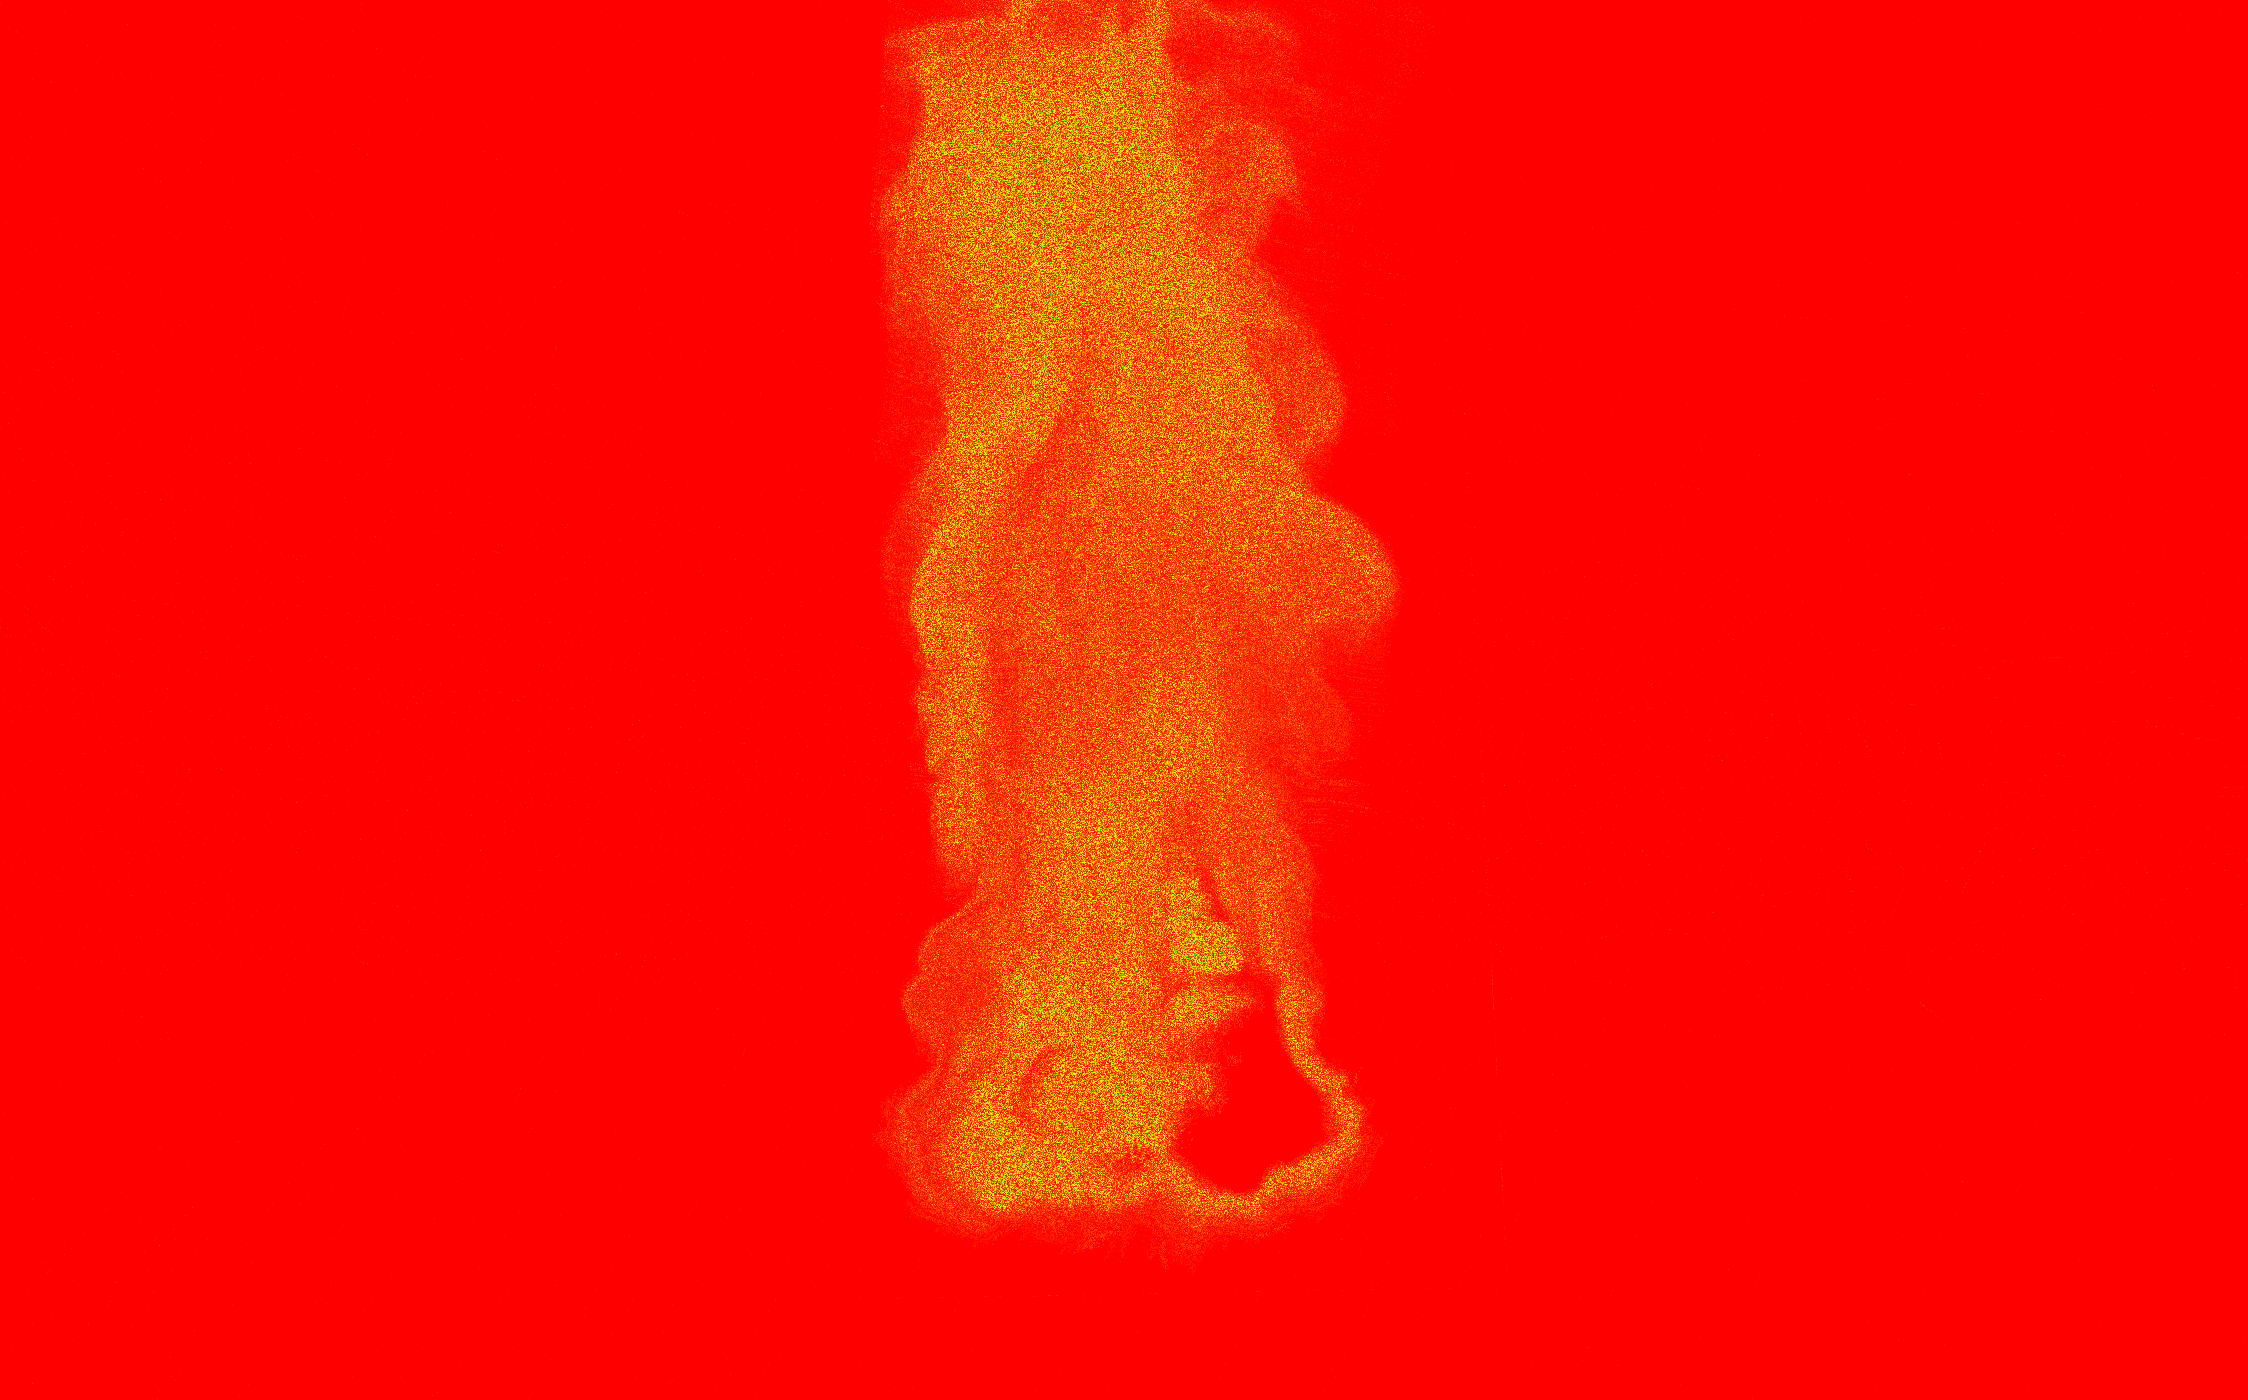
\includegraphics[width=0.3\textwidth]{compare_images_pytorch/diff_fire_format_f16.png} \label{fig:block_compression:fire_f16}
    }
    \hspace{0.2cm}
    \subfloat[Fire RMSE between 32-bit float and Unorm formats. We observe noise in the low-density regions at the top of the flame]{
        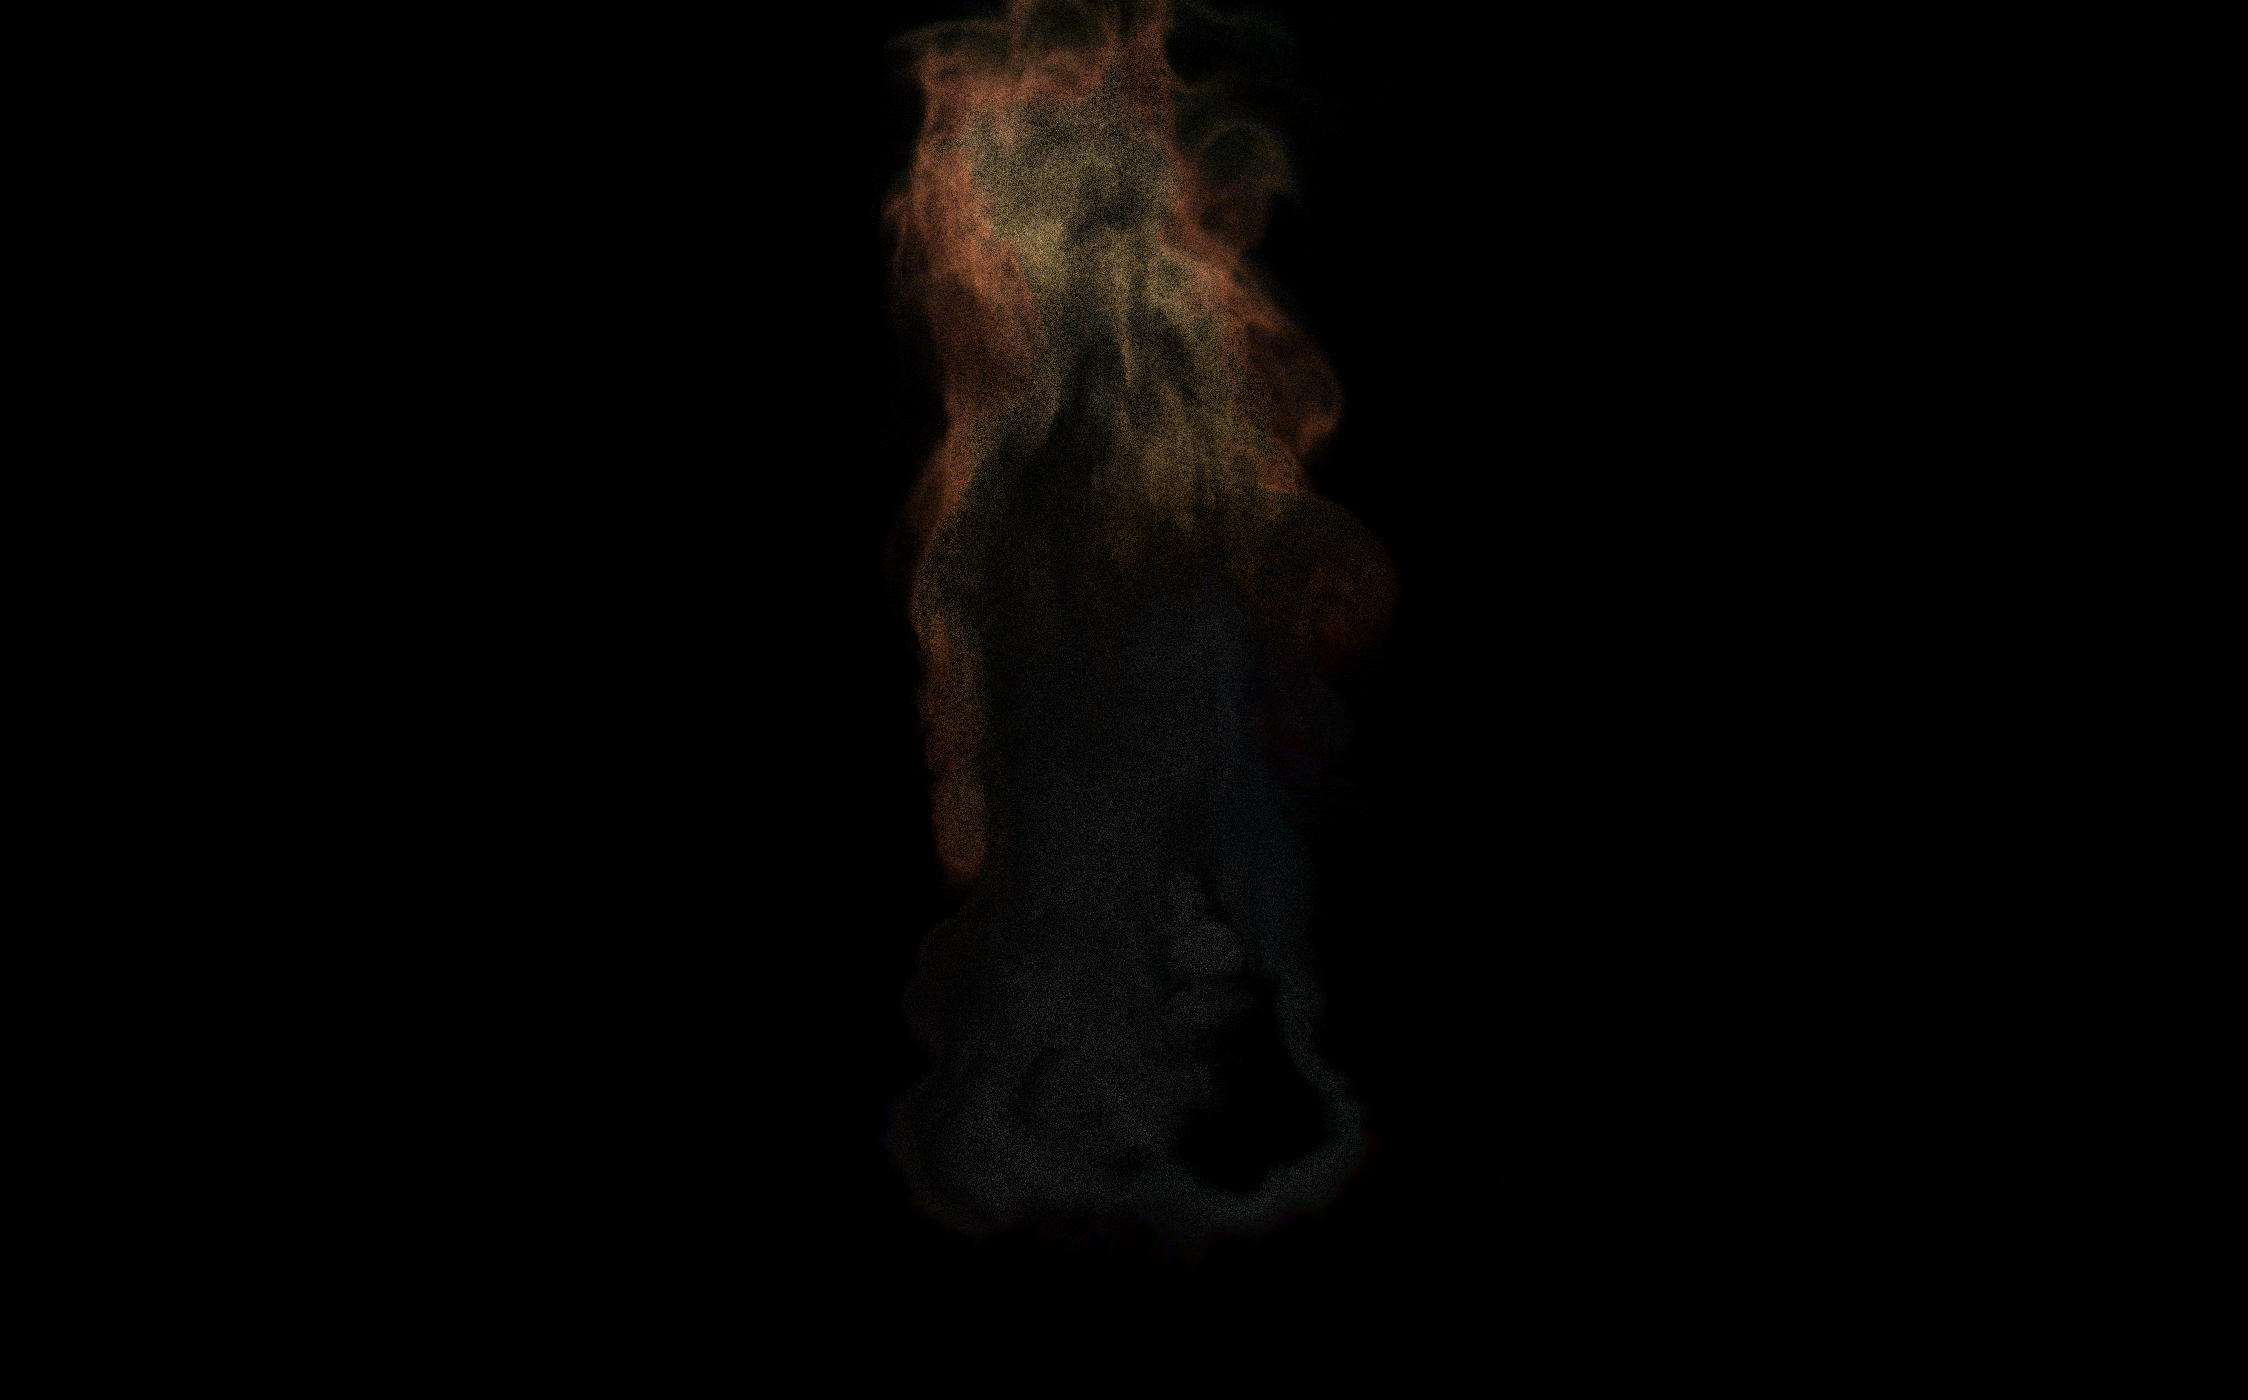
\includegraphics[width=0.3\textwidth]{compare_images_pytorch/diff_fire_format_unorm.png} \label{fig:block_compression:fire_unorm}
    }
    \hspace{0.2cm}
    \subfloat[Dragon RMSE between 32-bit float and BC7 formats. We only observe inherent path tracing noise.]{
        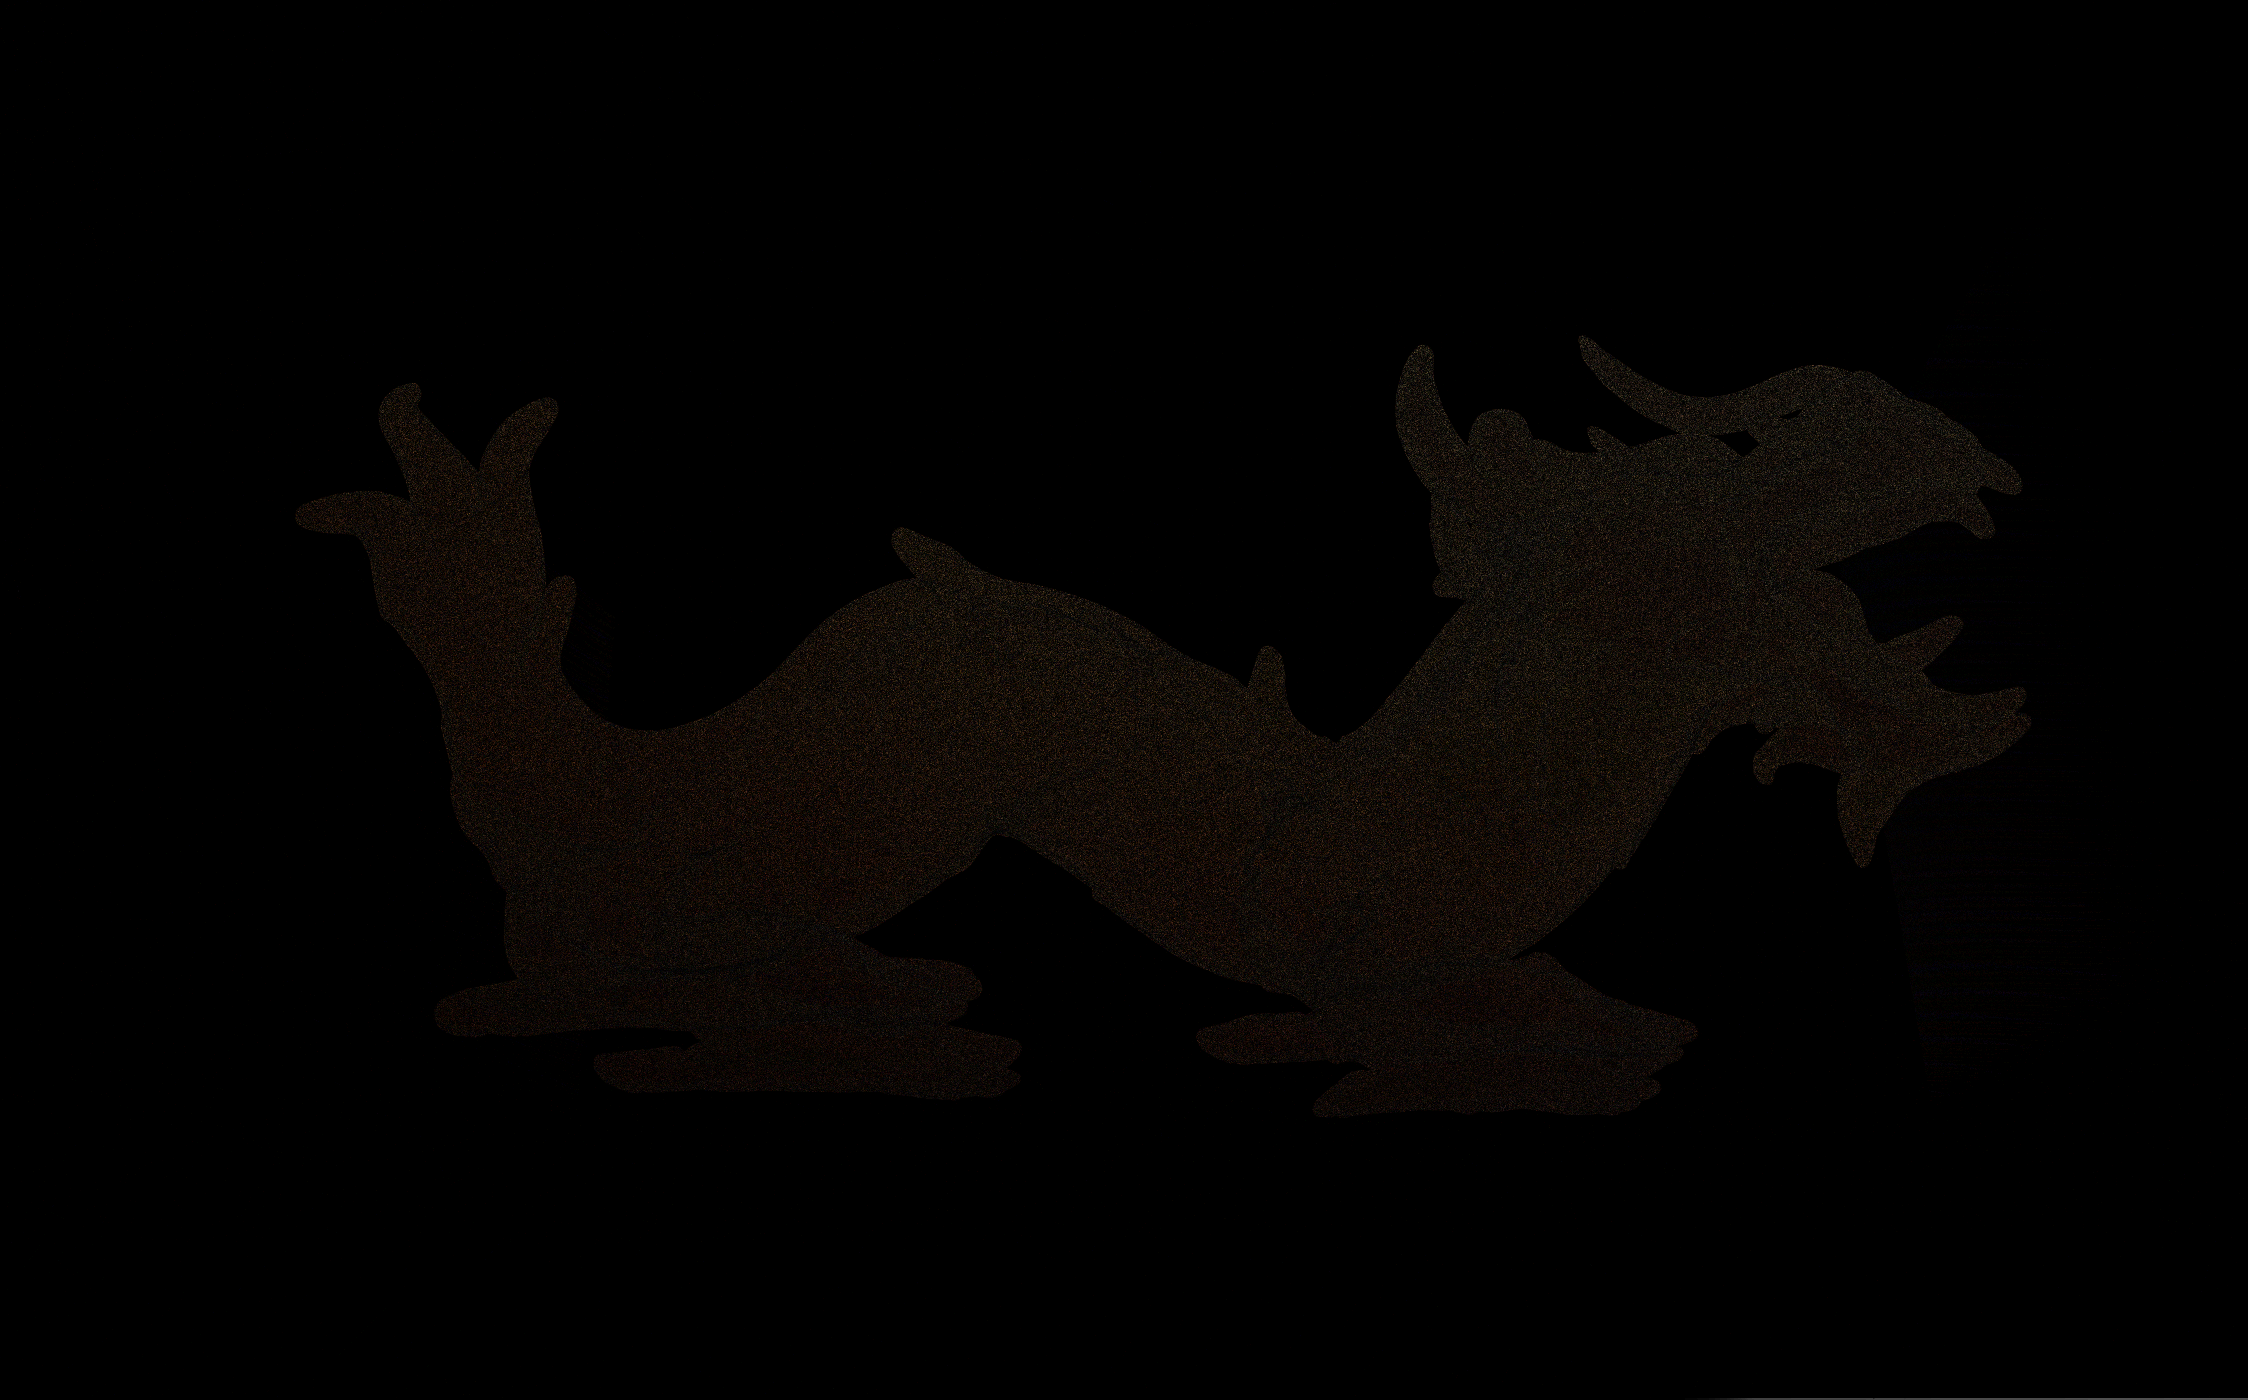
\includegraphics[width=0.3\textwidth]{compare_images_pytorch/diff_dragon_format_bc7.png} \label{fig:block_compression:dragon_bc7}
    }
    \hfill
    \subfloat[Table with the RMSE between 32-bit floating point  per voxel, and other data formats.]{

        \begin{tabular}{|l|l|l|l|}
            \hline
            \textbf{Model} & \textbf{Data Format} & \textbf{RMSE} \\
            \hline
            Bunny          & f16                  & 0.0048        \\
                           & Unorm                & 0.0050        \\
                           & bc7                  & 0.0050        \\
            \hline
            Disney Cloud   & f16                  & 0.0089        \\
                           & Unorm                & 0.0089        \\
                           & bc7                  & 0.0135        \\
            \hline
            Dragon         & f16                  & 0.0062        \\
                           & Unorm                & 0.0062        \\
                           & bc7                  & 0.0064        \\
            \hline
            Fire           & f16                  & 0.0044        \\
                           & Unorm                & 0.0099        \\
                           & bc7                  & 0.0100        \\
            \hline
        \end{tabular}
        \label{tab:compression_rmse}
    }

    \caption{The Root Mean Square Error (RMSE) of the compression of four different models at $1000$ samples per pixel with 32-bit floats per voxel used as a baseline. Red pixels have a low error and higher hue values (more green/blue) indicate a larger error. Higher samples per pixel counts reduce the inherent path tracing noise which changes the RMSE offset seen in the comparison with f16 (this format is practically identical to f32), however, converging properly with tens of thousands of samples was impractical. We calculate the difference against the full 32-bit floating point precision model as this is closest to the ground truth.} \label{fig:block_compression}
\end{figure}


\begin{figure}[H]
    \centering
    \subfloat[Disney Cloud without cluster compression.]{
        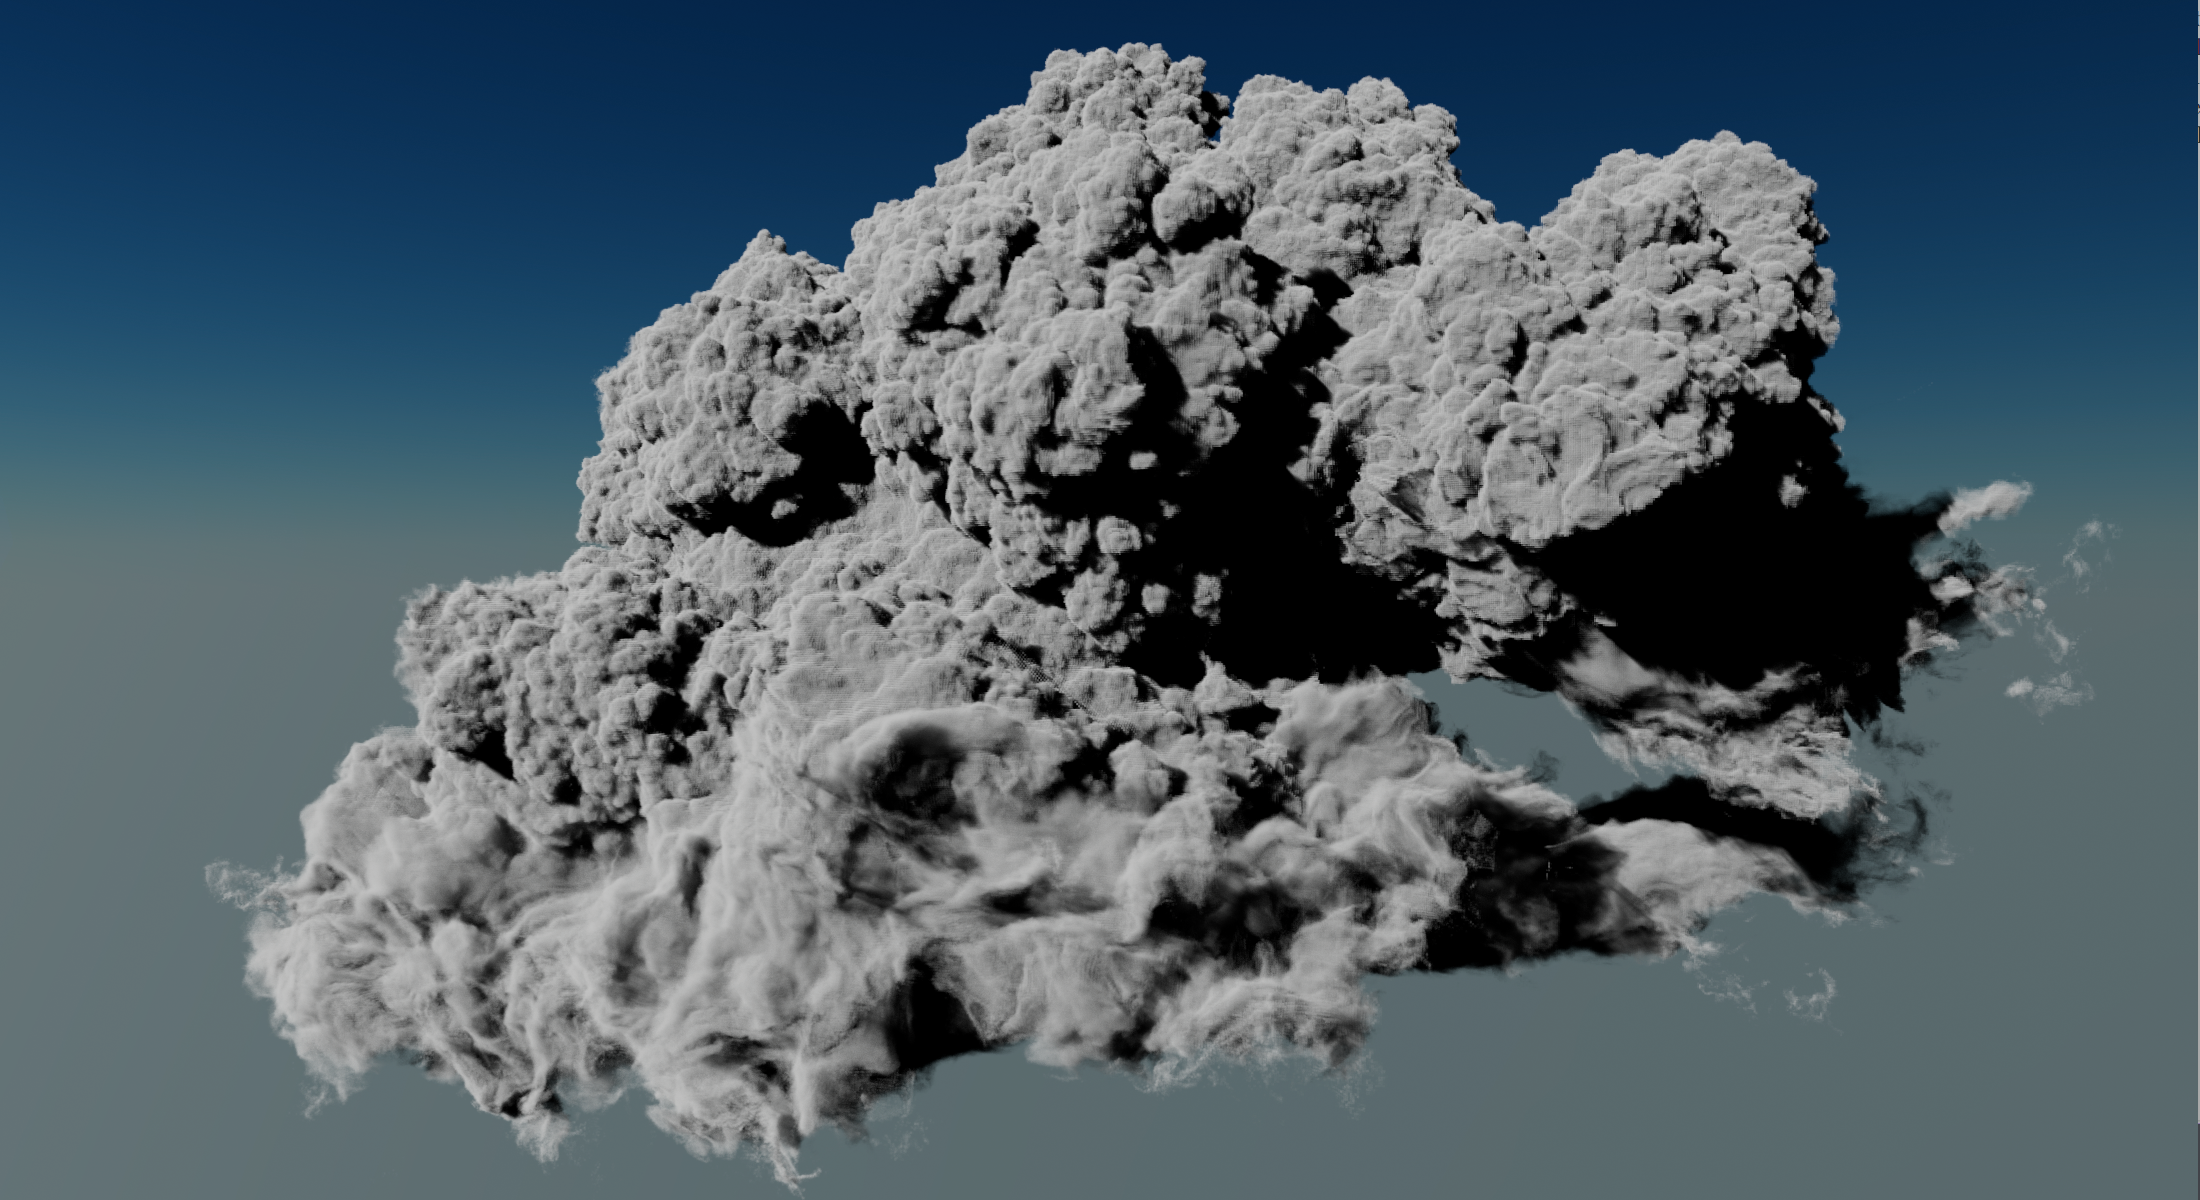
\includegraphics[width=0.45\textwidth]{figures/disney_cloud_clustering_raw.png} \label{fig:block_compression_visualized:raw}
    }
    \hfill
    \subfloat[Disney Cloud with all bricks being clustered.]{
        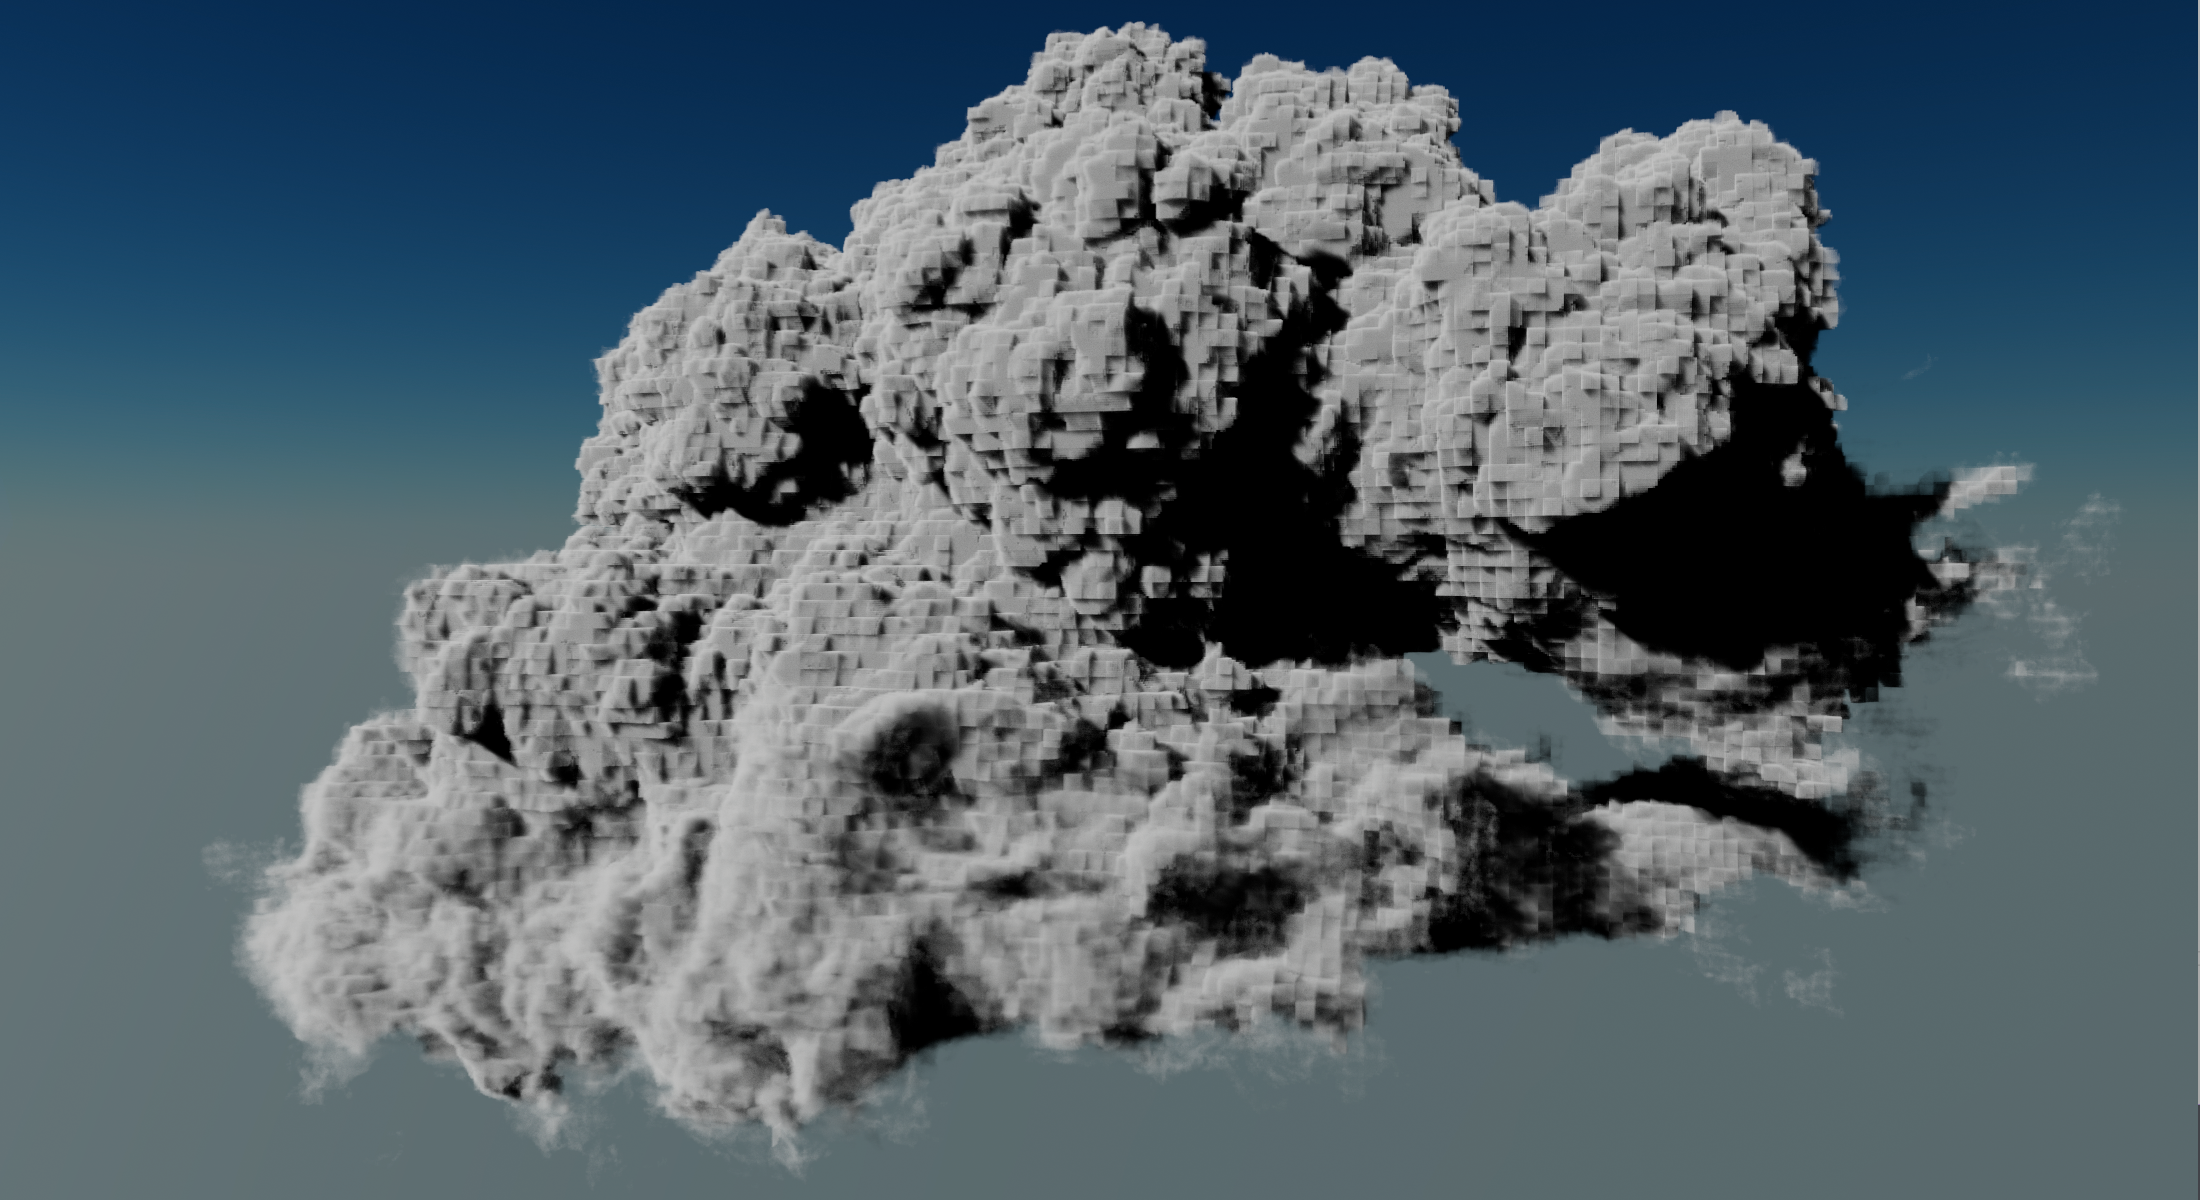
\includegraphics[width=0.45\textwidth]{figures/disney_cloud_clustering_99.png} \label{fig:block_compression_visualized:99}
    }
    \hfill
    \subfloat[Disney Cloud with a variance reduction of $0.1$, clustering roughly $70\%$ of the bricks into 100 new bricks.]{
        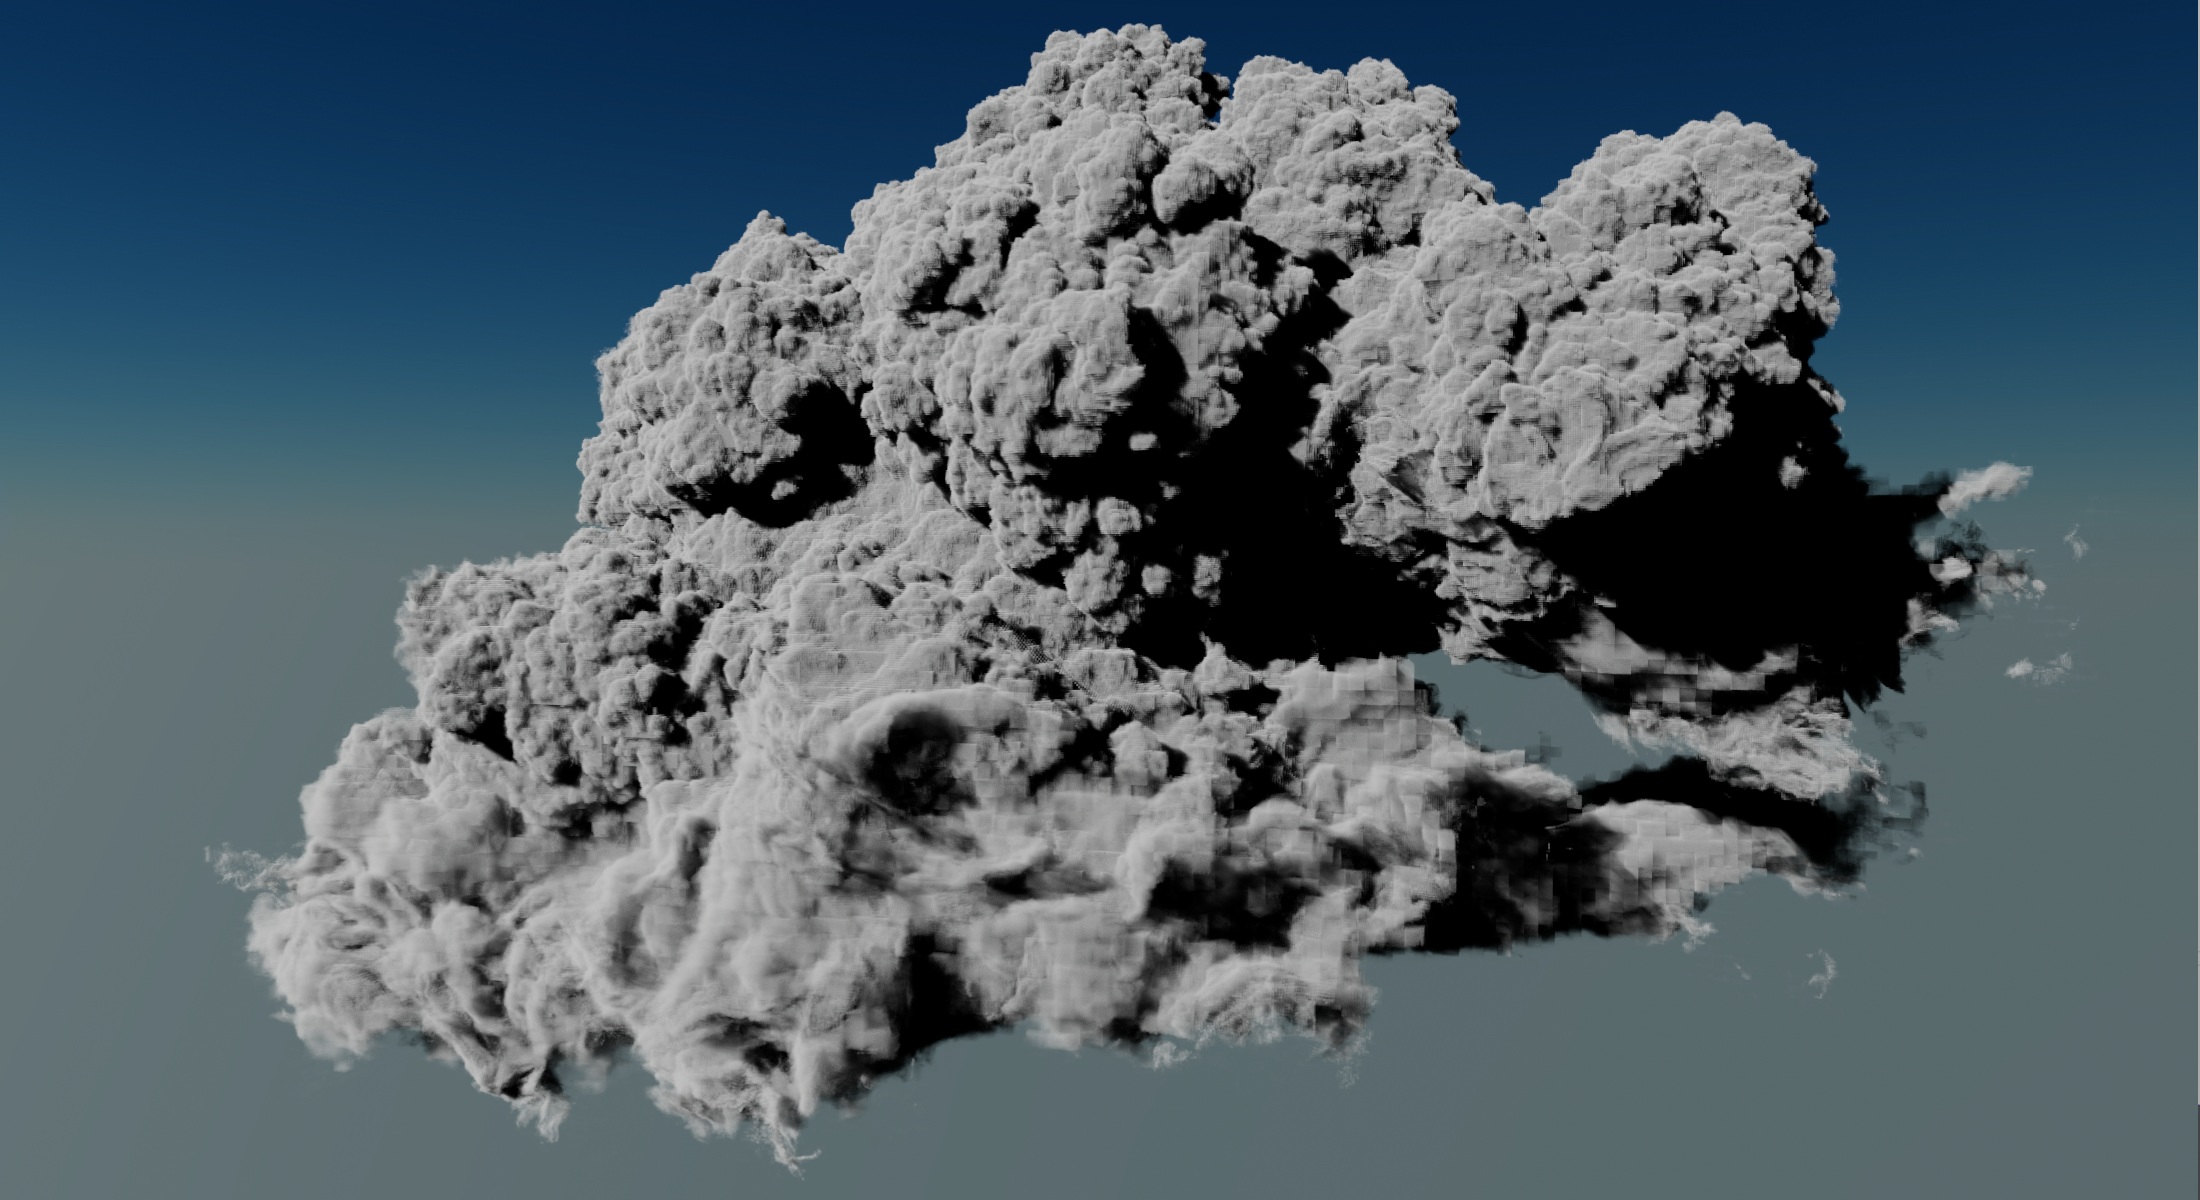
\includegraphics[width=0.45\textwidth]{figures/disney_cloud_clustering_1.png} \label{fig:block_compression_visualized:1}
    }
    \hfill
    \subfloat[Disney Cloud with a variance reduction of $0.01$, clustering roughly $35\%$ of the bricks into 100 new bricks.]{
        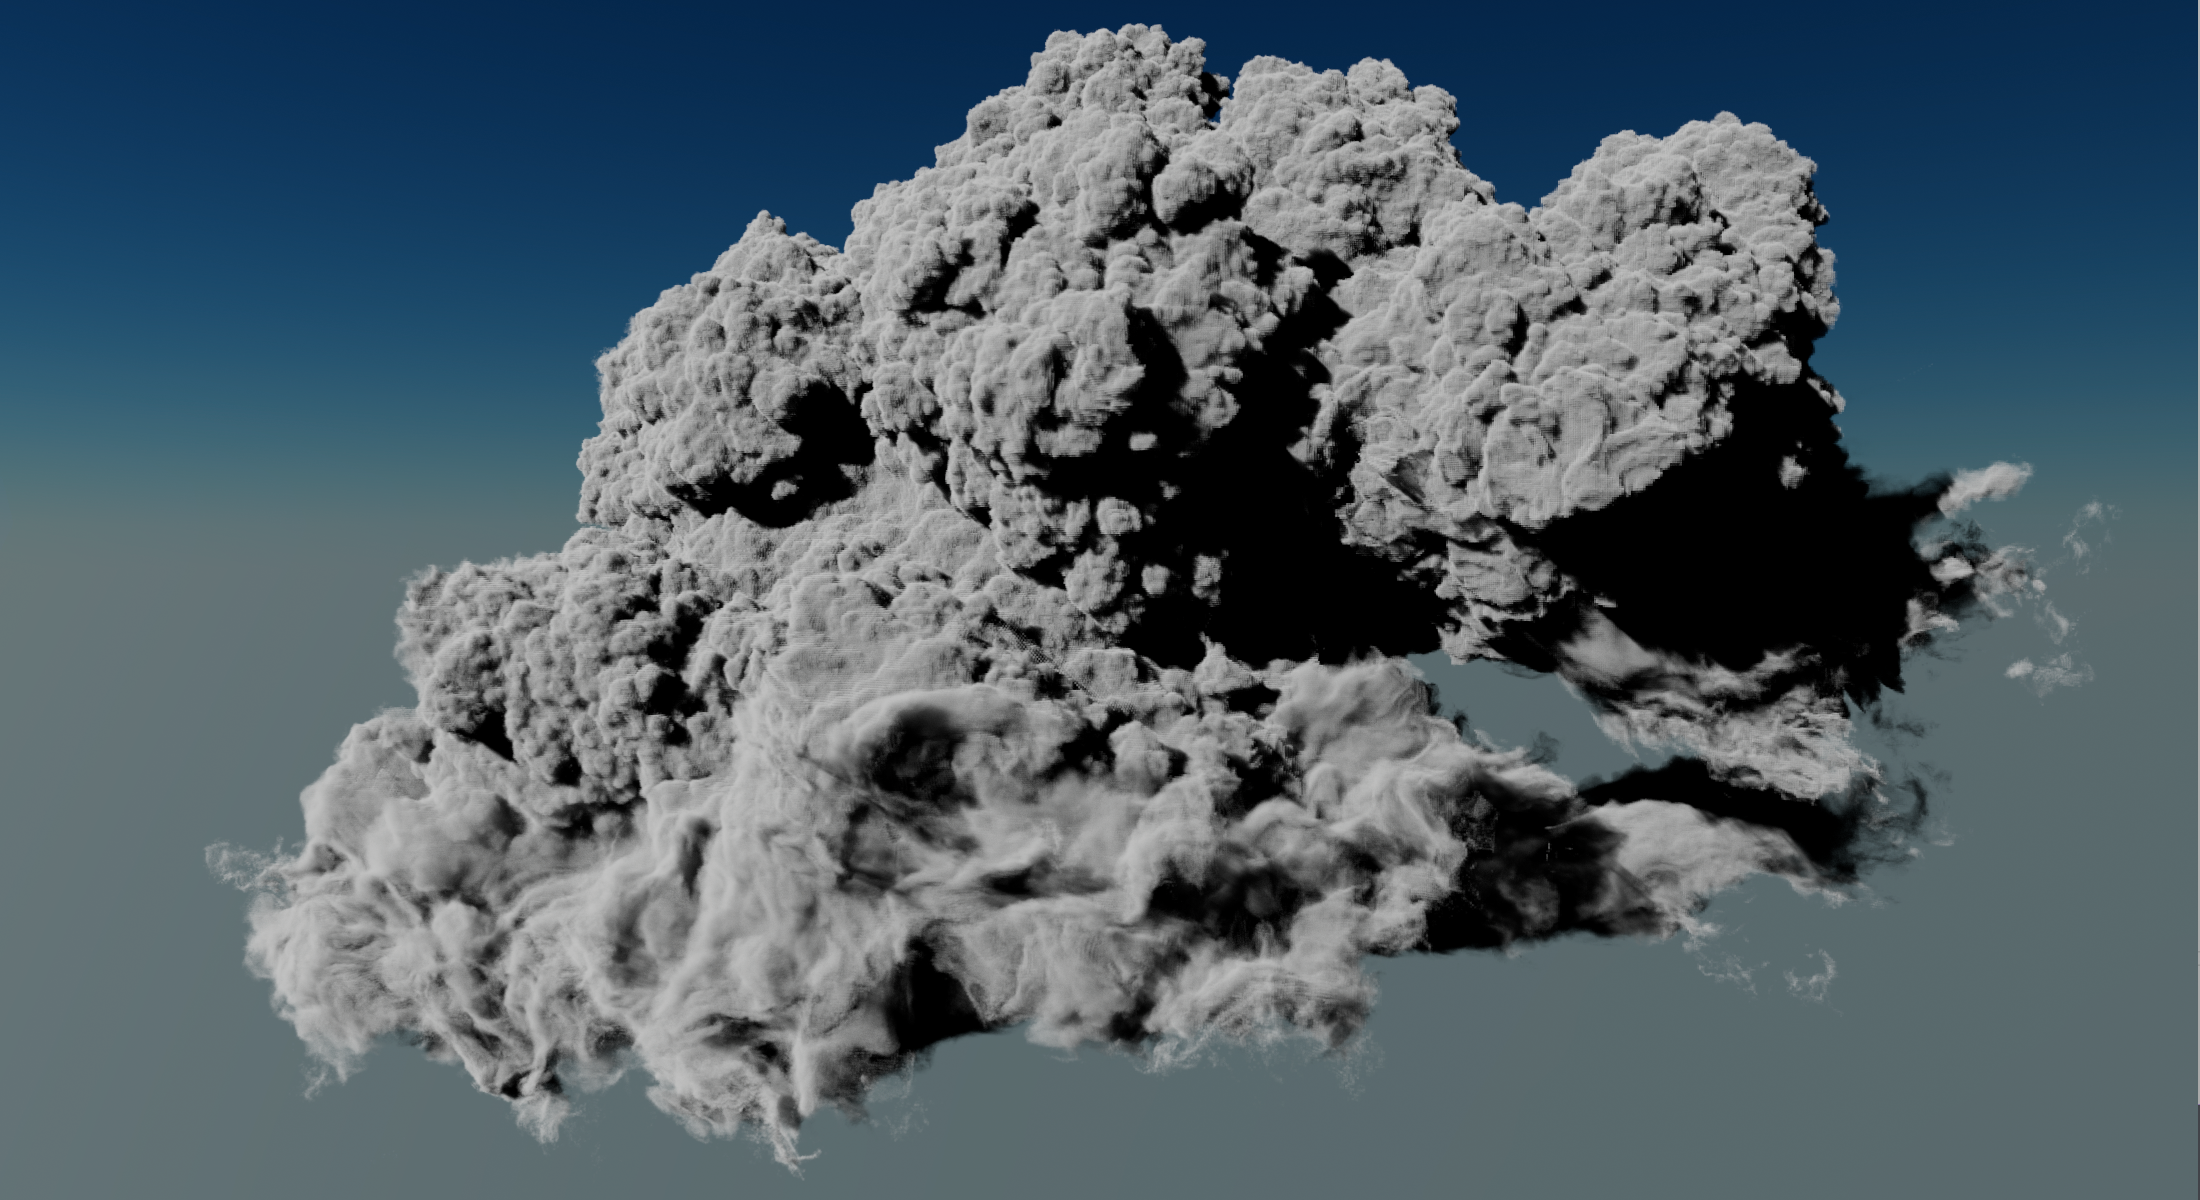
\includegraphics[width=0.45\textwidth]{figures/disney_cloud_clustering_01.png} \label{fig:block_compression_visualized:01}
    }
    \hfill
    \subfloat[The input parameters $k$, Iterations and Variance Threshold, with their respective compression results.]{

        \begin{tabular}{|l|ccc|cccc|}
            \toprule
            \hline
            Model        & $k$  & Iterations & Variance Threshold & Before  & After   & Compression Ratio & RMSE            \\
            \hline
            \midrule
            Shockwave    & 1000 & 5          & 0.01               & 1877783 & 1621453 & 0.86349           & 0.0151          \\
                         & 100  & 10         & 0.01               & 1877783 & 1620553 & 0.86301           & 0.0151          \\
                         & 100  & 5          & 0.1                & 1877783 & 100     & 0.00005           & 0.0425          \\
                         & 100  & 5          & 0.01               & 1877783 & 1620553 & 0.86301           & \textbf{0.0046} \\
            \hline
            \midrule
            Dragon       & 1000 & 5          & 0.1                & 123934  & 67031   & 0.54086           & \textbf{0.0077} \\
                         & 100  & 10         & 0.1                & 123934  & 66131   & 0.53359           & 0.0092          \\
                         & 100  & 5          & 0.01               & 123934  & 66131   & 0.53359           & 0.0096          \\
                         & 100  & 5          & 0.1                & 123934  & 66131   & 0.53359           & 0.0093          \\
                         & 100  & 5          & 0.99               & 123934  & 66131   & 0.53359           & 0.0279          \\
            \hline
            \midrule
            Disney Cloud & 1000 & 5          & 0.1                & 275730  & 73456   & 0.266405          & 0.227           \\
                         & 100  & 10         & 0.1                & 275730  & 72556   & 0.26314           & 0.0299          \\
                         & 100  & 5          & 0.01               & 275730  & 178663  & 0.64796           & \textbf{0.0088} \\
                         & 100  & 5          & 0.1                & 275730  & 72556   & 0.26314           & 0.0283          \\
                         & 100  & 5          & 0.99               & 275730  & 100     & 0.00036           & 0.0659          \\
            \hline
            \midrule
            Chimney      & 1000 & 5          & 0.1                & 915701  & 27820   & 0.03038           & 0.0109          \\
                         & 100  & 10         & 0.1                & 915701  & 26920   & 0.02939           & 0.0138          \\
                         & 100  & 5          & 0.01               & 915701  & 401147  & 0.43807           & \textbf{0.0046} \\
                         & 100  & 5          & 0.1                & 915701  & 26920   & 0.02939           & 0.0131          \\
                         & 100  & 5          & 0.99               & 915701  & 100     & 0.00010           & 0.0185          \\
            \hline
            \bottomrule
        \end{tabular}
        \label{tab:block_compression_visualized:table}
    }

    \caption{The results of clustering-based compression. Four models were used for the comparison of the different clustering parameters. The tweakable clustering parameters are $k$, The number of iterations and the variance threshold. These are then used to cluster our brick data. The \textit{Before} and \textit{After} columns show the brick count. $Ratio$ is the ratio between brick numbers before and after clustering. The RMSE is calculated using one of the frames for each model. All comparisons are done with BC7 compression enabled.} \label{fig:block_compression_visualized}
\end{figure}

\begin{figure}[H]
    \centering
    \subfloat[Texture voxel brick data before clustering.]{
        \includegraphics[width=0.45\textwidth]{figures/pre_clustered_memory.png} \label{fig:implementation:compression:pre_cluster}
    }
    \hfill
    \subfloat[Texture voxel brick data after clustering.]{
        \includegraphics[width=0.45\textwidth]{figures/post_clustered_memory.png} \label{fig:implementation:compression:post_cluster}
    }
    \caption{The results of our clustering compression technique. All of these results use Bc7 encoding. Figure \ref{fig:implementation:compression:pre_cluster} shows a slice out of the voxel brick data texture on the GPU. There are visible long chains of black or otherwise greyscale slices which means that these bricks are mostly homogeneous inside that brick. In Figure \ref{fig:implementation:compression:post_cluster} we again see a slice of the voxel brick data texture, but this time after running our clustering algorithm. There are visibly fewer patches of grayscale bricks when compared to Figure \ref{fig:implementation:compression:pre_cluster}. This shows us that we are removing homogeneous bricks, and keeping unique nodes.} \label{fig:implementation:compression:cluster}
\end{figure}



\begin{figure}[H]
    \subfloat[Level set rendering the depth of the primary hit calculated with HDDA.]{
        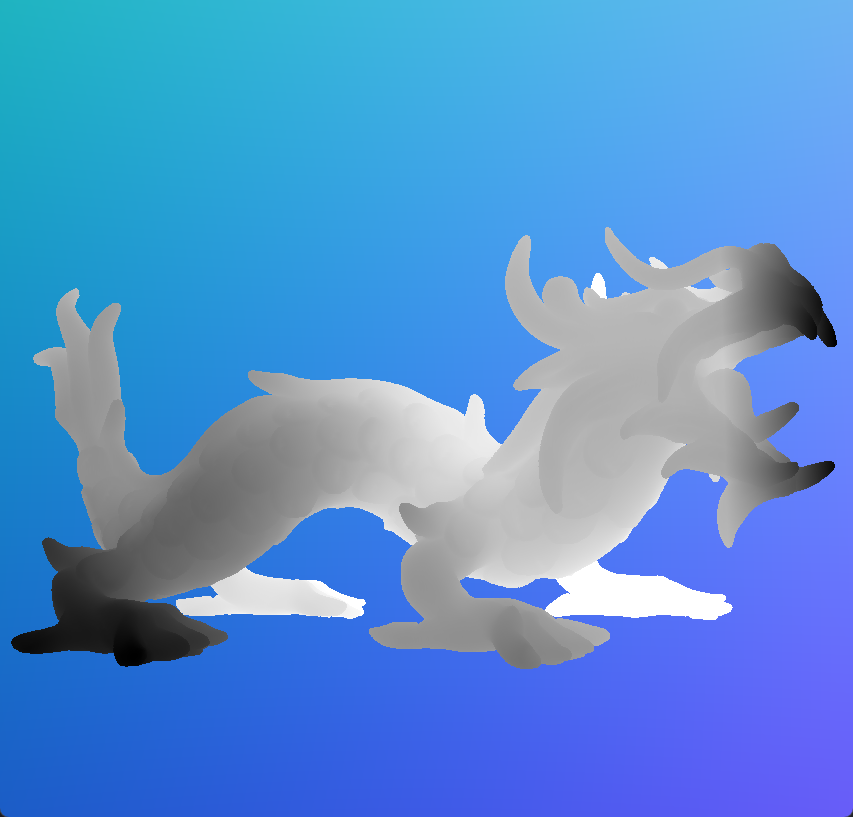
\includegraphics[width=0.45\textwidth]{figures/dragon_levelset.png} \label{fig:tracing_performance:level_set}
    }
    \hfill
    \vspace{0.5cm}
    \subfloat[Fog volume rendering the accumulated density along the ray path.]{
        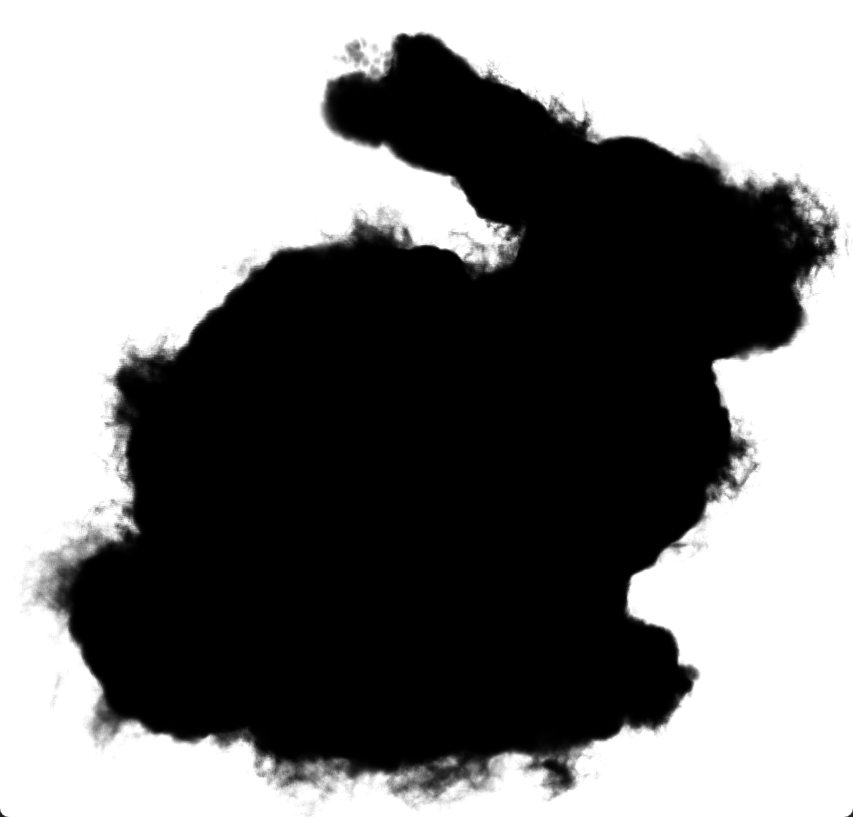
\includegraphics[width=0.45\textwidth]{figures/bunny_fogvolume.png} \label{fig:tracing_performance:fog_volume}
    }
    \hfill
    \subfloat[Performance numbers between NanoVDB from \cite{NanoVDBBenchmark} and our implementation. All numbers are in milliseconds.]{
        \begin{tabularx}{\textwidth}{|c|X|X|X|X|X|X|}
            \hline
            \textbf{Method} & \textbf{Fog Volume} & \textbf{SM Occupancy} & \textbf{L1 pressure} & \textbf{Level Set} & \textbf{SM Occupancy} & \textbf{L1 pressure} \\
            \hline
            NanoVDB         & $4.971$             & ?                     & ?                    & $2.427$            & ?                     & ?                    \\
            \hline
            Ours            & $9.815$             & $95.9\%$              & $30.9\%$             & $1.092$            & $62.1\%$              & $36.6\%$             \\
            \hline
        \end{tabularx}
        \label{tab:tracing_performance:numbers}
    }
    \caption{We attempted to benchmark using the same setup as \cite{NanoVDBBenchmark}. Unfortunately, they did not provide a thorough explanation of the benchmark beyond the resolution and the models which were used, these are shown in \ref{fig:tracing_performance:fog_volume} and \ref{fig:tracing_performance:level_set}. We do not know how exactly the models were placed in the NanoVDB benchmark, so we positioned the objects to cover as much of the screen as possible to capture the lower bound of the ray tracing performance. In Table \ref{tab:tracing_performance:numbers} we show the fog volume and level set render timings in ms. We also show the streaming multiprocessor (SM) occupancy and the L1 pressure. These two metrics provide insight into bottlenecks and potential future optimization targets. Unfortunately these detailed performance metrics were not provided with the NanoVDB results, thus these fields are highlighted with questionmarks.}
    \label{tab:tracing_performance}
\end{figure}